\chapter{System Architecture} \label{ch:system-architecture}
\markboth{System Architecture}{}

\paragraph{}
We propose to tackle system redundancy in both the IoT Edge \& Cloud layer by designing an architecture where IoT Edge \& Cloud systems of different stakeholders can dynamically enter into a federation, agreeing that in case of one’s failure (degraded \gls{stakeholder}), the other stakeholder will kick-start a mechanism in order to conduct \gls{iot-management} of the (degraded stakeholder’s) devices. This is a dynamic process, where the systems have access to a centralized marketplace in order to find the optimum option. While our research and implementation focused on the IoT Edge layer, the exact principles can be applied in the cloud layer, although the actual parameters and implementation rest outside of the scope of this work.

In this Chapter we will go through the principles of the proposed architecture and discuss on the core technologies  we choose as the basis of the architecture. We will firstly address the architecture as a whole, starting with the main architectural paradigm, that of micro-services. We then proceed to talk about the technology that enables the provision of resources to run 3rd party services on the same hardware(i.e container technology). Finally, we will delve into the two main subsystems, that is the IoT Edge and the Cloud and their respective modules.

The proposed architecture is intended to serve as a high-level overview of the envisaged components and processes. The specification of each component and core activity, such as the algorithms and state machines, are expected to be presented in a future work. Moreover, we choose to focus on a narrow aspect for the architecture in order to realise our proof of concept, implementing only the core modules of this architecture.

\section{Proposed Architecture}

\begin{figure}[h]
    \centering
    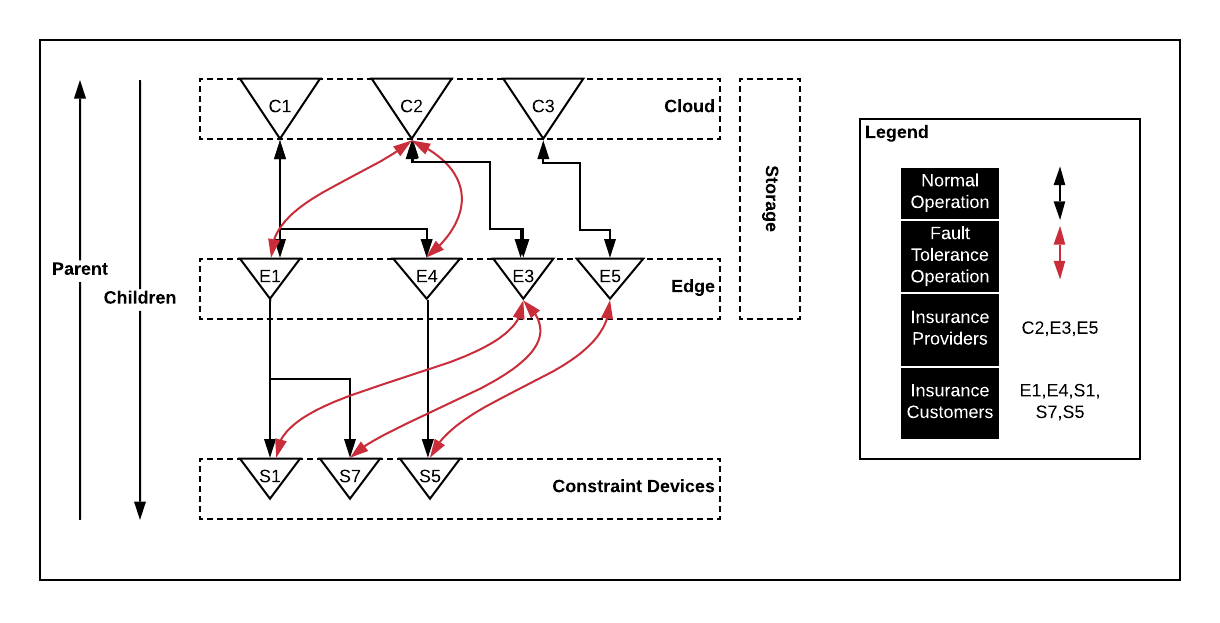
\includegraphics[width=1\textwidth]{images/layer-fault-tolerant.png}
    \caption{The hierarchy layered architecture during normal and fault-tolerance operation}
    \label{fig:hier-fault}
\end{figure}

Figure \ref{fig:hier-fault} outlines the hierarchy and layering of the proposed system design. The normal operation illustrates an \gls{iot-connection} between devices that belong to the same stakeholder (“owner”), while the “Fault-Tolerance” operation illustrates a connection between devices that belong to different stakeholders, and thus there is an exchange of service/value.
 
For each stakeholder’s cloud, his IoT Edge devices are considered his \textbf{children} and the sensors of each IoT Edge system are the \textbf{children} of that particular Edge. 

\begin{figure}[h]
    \centering
    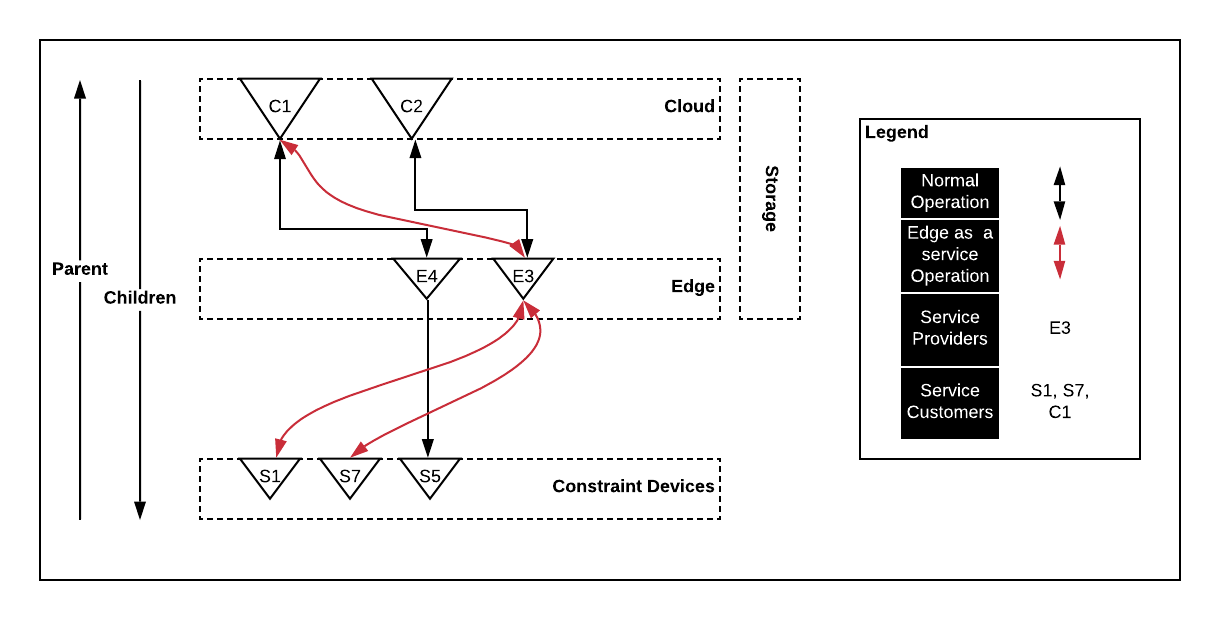
\includegraphics[width=1\textwidth]{images/layer-service-provision.png}
    \caption{The hierarchy layered architecture during "IoT Edge as a service" Operation}
    \label{fig:hier-service}
\end{figure}

Figure \ref{fig:hier-service} shows the same hierarchy but in a more generic scenario, that of the “IoT Edge as a Service” or “EaaS”.  The normal operation illustrates a connection between devices that belong to the same stakeholder (“owner”), while the “IoT Edge as a service” operation illustrates a connection between devices that belong to different stakeholders, and thus there is an exchange of service/value.

The stakeholder owner of cloud system \textit{C1} and sensors \textit{S1,S7} needs an IoT Edge Computing device to manage his sensors \textit{(S1, S7)}, aggregate their data, pre-process them and lastly forward them to the Cloud \textit{(C1)}. Edge \textit{E3} offers such services, while at the same time it offers services to \textit{C2} which belongs to the same stakeholder as \textit{E3}. In other words, \textit{E3} dynamically and while continuing it’s operations, procures resources as requested by \textit{C1}. In this scenario, since we assume that \textit{S1, S7} are managed entirely by another’s stakeholder Edge device, we say that \textit{S1, S7} are the children of \textit{E3} (albeit for a certain period). \gls{iot-management} is a generic term that includes all the relevant IoT activities a parent device must perform to the children, such as provisioning, aggregation, actuating and others.

\section {Decoupling the Storage Layer}

The System is divided in 4 main subsystems layers (Storage, Cloud, Edge, Sensors).  We chose to add an additional layer to that of the IoT reference 3 tier architecture\cite{tranoris}, that of the Storage. By decoupling the storage layer from the cloud layer-which is usually part of-we envision a system where both Cloud \& IoT Edge systems, use the same long-term storage layer, facilitating the high availability functionality we envision. The entire state of the IoT Edge system is foreseen to be stored in the storage layer, both in terms of application logic and sensor data, at specific intervals. Thus, a IoT Edge Node could be easily replicated while maintaining access to important sensor data. 

\textbf{Coupling} is frequently used in software engineering as a metric for the quality of the program in development. It expresses the degree of interdependence between software modules; how closely two modules are connected and how strong their relationship is.  Two loosely coupled (or decoupled) systems can change independently without having any ripple effects one to another. Moreover, they are easily replaceable and the overall quality of the system is increased.

Considering the same stakeholder/owner, a Cloud is the Parent of multiple Edges and an IoT Edge is the Parent of multiple Sensors. The system is agnostic regarding the Storage and Sensor (Constraint Devices)  layers, as long as they follow the specifications established by the relevant hardware and interfaces. 

In our analysis, the system stakeholder can be divided into two groups:
\begin{itemize}
    \item Service-Provider : The owner of the physical IoT Edge device that procures some of it’s resources to run services of 3rd parties. In the use-case implementation, the service-provider  is the Insurance Provider (since the service is a fault-tolerance insurance).
    \item Service-Customer: The stakeholder who requests to the service-provider  to run a number of services on the IoT Edge of the service-provider . In the use-case implementation, the Service Customer is the Insurance Customer (since the service is a fault-tolerance insurance).
\end{itemize}



\section{A design based on Microservices}

Microservices are a software engineering technique, a variant in essence of the Service Oriented Architecture (SOA). It defines that an application is structured as a collection of loosely coupled services\cite{8354433}, which are extremely fine-grained implementing lightweight communication protocols. A service in a SOA usually have 4 main properties \cite{service-oriented-architecture}:
\begin{enumerate}
    \item It logically represents a business activity with a specified outcome.
    \item It is self-contained.
    \item It is a black box for its consumers.
    \item It may consist of other underlying services.
\end{enumerate}

This architecture boosts modularity, since each service can be replaced, updated or change without affecting the overall system. Moreover, since each service is independent, it facilitates the understanding of the system (since each service is viewed as an autonomous micro-system), it boosts development speed as teams can develop services in parallel and facilitates deployment and continuous integration (CI) \cite{microservices.io}.

Microservices usually communicate over a local network using a technology-agnostic protocol, more commonly HTTP. They are independently deployable and more importantly can be developed using different programming technologies, databases and in general heterogenous technologies, as long as the interfaces match in protocols and structure. 

They are commonly found in cloud-native applications using the container technology to facilitate deployment, a method that was followed in our solution. Finally, it is worth noting that a microservice cannot be part of a monolithic application. Rather it is a self-contained piece of business functionality with clear interfaces, and may, through its own internal components, implement a layered architecture. From a strategy perspective, microservices architecture follows the Unix philosophy of "Do one thing and do it well"\cite{krause2015microservices}.

\subsection{Why Microservices}

The microservices paradigm was chosen for 2 main reasons:
\begin{enumerate}
    \item Our goal is to create a platform where an agent (i.e user, device)  can rent resources to run services on a 3rd party IoT Edge device. Having a microservices architecture, it is extremely easy to implement a platform where services can be added and remove on an ad-hoc basis, without affecting the overall functionality of the system.
    \item The system was built around the EdgeX Foundry Internet of Things platform. EdgeX foundry architecture is that of microservices, so it was easier to integrate our custom modules to an already established IoT platform, which we will describe in the following Subsection \ref{sub:edgex}.
\end{enumerate}

\subsection{EdgeX Foundry} \label{sub:edgex}

EdgeX Foundry\cite{edgex-foundry} is a vendor-neutral open source project, under the auspices of the Linux foundation. It builds a common open framework for IoT Edge Computing in the domain of Internet of Things. At the core of the initiative,lies an interoperability framework hosted within a full hardware and OS agnostic reference software platform. It enables an ecosystem of plug-and-play components that unifies the existing IoT Edge marketplace and accelerates the development and deployment of Internet of Things solutions.

The project was spearheaded by Dell in 2017 and later open sourced under Linux Foundation. Several companies (such as Dell, Redis, and others) are actively contributing to the project which also has a vibrant community. 

\begin{figure}[h]
    \centering
    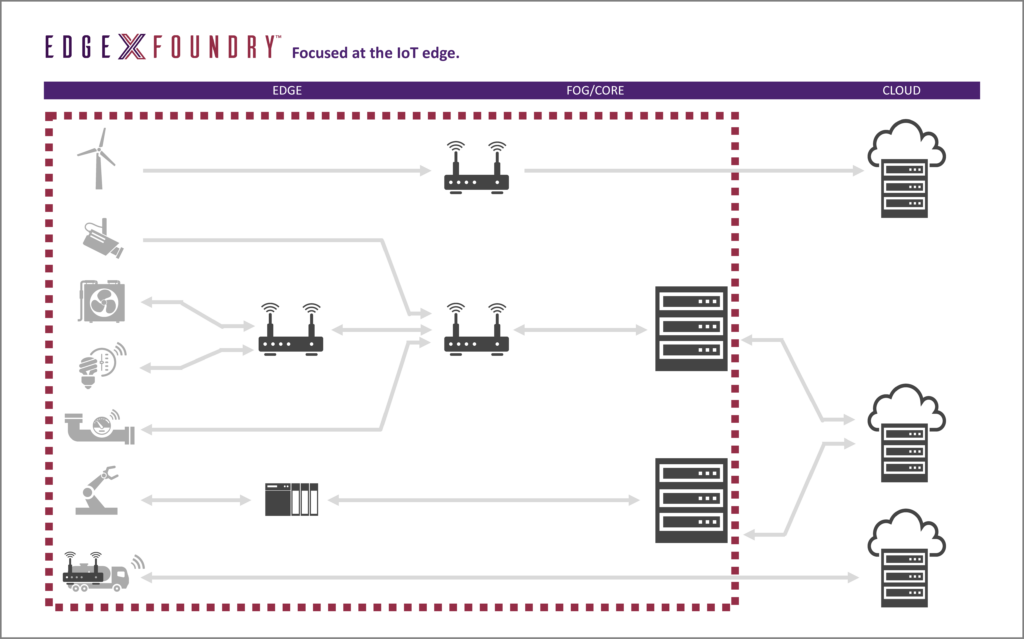
\includegraphics[width=0.6\textwidth]{images/edgex_arch1.png}
    \caption{The project focus of EdgeX Foundry in the IoT stack}
    \label{fig:edgex_focus}
\end{figure}

EdgeX foundry focuses on the Industrial IoT Edge, shown in Figure \ref{fig:edgex_focus} leveraging cloud-native principles, such as loosely-coupled microservices and platform independence, to architect around the needs of the IoT Edge. It mainly targets IoT Edge Nodes such as gateways, routers and embedded PCs and their interoperability. It can run on a single IoT Edge or be distributed over a larger number.

\begin{figure}[h]
    \centering
    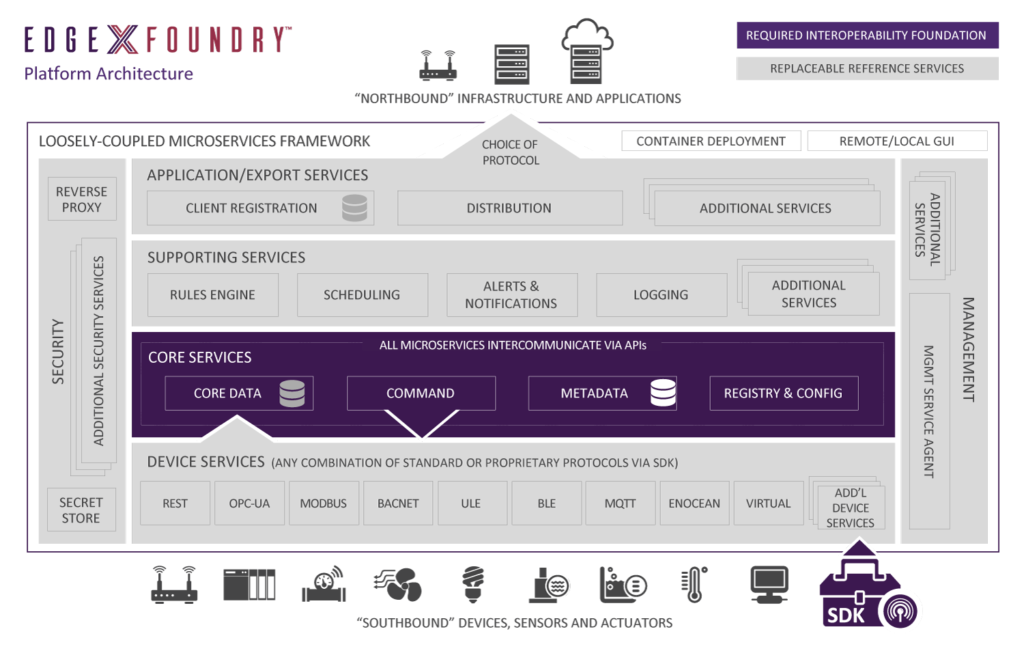
\includegraphics[width=0.9\textwidth]{images/edgex_arch.png}
    \caption{The EdgeX high-level architecture}
    \label{fig:edgex_arch}
\end{figure}

Figure \ref{fig:edgex_arch} illustrates the EdgeX platform architecture, each square indicates a different microservice, which are grouped based on their functionality in the platform. A user can select to run only a subset of the available microservices, except for the core services (Purple) which are needed as a whole. The device service SDK\cite{device-service-sdk} is needed to interface any Constrained Device to the platform.

The grey microservices are reference services that constitute a fully functional IoT Edge software, but they are optional. EdgeX is fully agnostic concerning the \gls{north-side} and \gls{south-side} of the platform, as such we can even create a layered architecture of multiple EdgeX that perform different functionalities, as shown in Figure \ref{fig:edgex_fog_layer}.

EdgeX foundry is currently under heavy development and the reference implementation is in Go. The microservices communicate using HTTP and each has its own \acrfull{rest} interface resource. The suggested deployment method is using Docker Containers, as further discussed in Implementation Chapter \ref{ch:implementation}.

\begin{figure}[h]
    \centering
    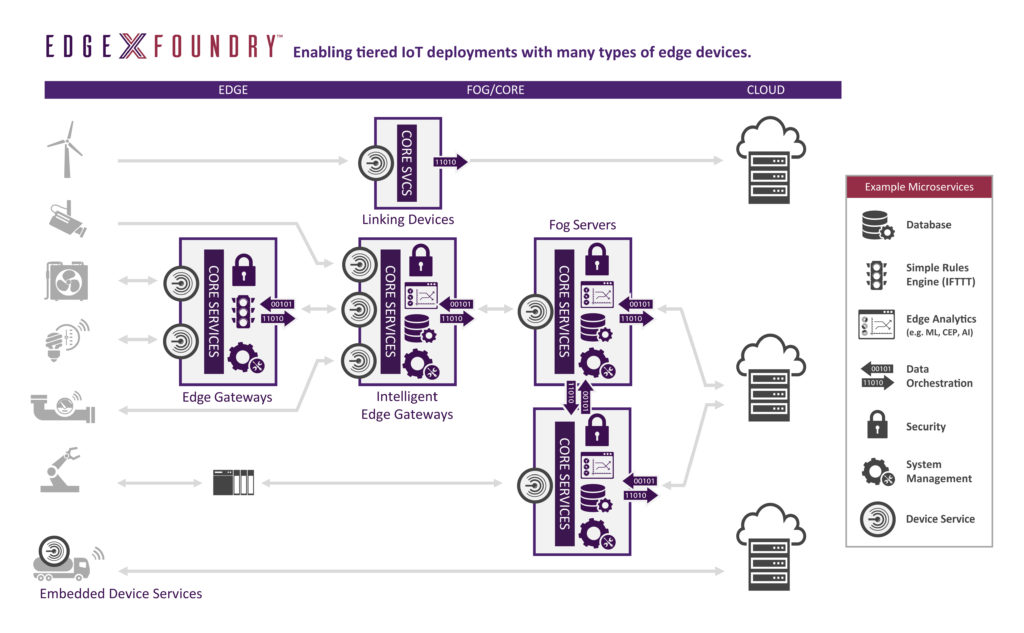
\includegraphics[width=0.9\textwidth]{images/edgex_fog_layer.jpg}
    \caption{A layered approach of fog computing using EdgeX}
    \label{fig:edgex_fog_layer}
\end{figure}

Below we give an apt description of each microservice so the reader better understand our implementation choices, where we choose to deploy only a subset of the available EdgeX foundry microservices.
 
\textbf{Core Services (CS)}
They separate the north and south side layers at the edge. Core services include the following components:
\begin{itemize}
    \item Core data: a persistence repository and associated management service for data collected from the south side objects.
    \item Command: a service that facilitates and controls actuation requests from the north side to the south side.
    \item Metadata: a repository and associated management service of metadata about the objects that are connected to EdgeX Foundry. It provides the capability to provision new devices and pair them with their owning device services.
    \item Registry and Configuration: provides other EdgeX Foundry microservices with information about associated services within EdgeX Foundry and microservices configuration properties. 
\end{itemize}

\textbf{Supporting Services (SS)}
The Supporting Services (SS) Layer encompass a wide range of microservices that provide the IoT Edge analytics and intelligence, and provide service to EdgeX Foundry itself. Normal software application duties such as logging, scheduling, and data clean up (scrubbing) are performed by microservices in the SS Layer. The rules engines, alerting and notification microservices are within the SS Layer because they operate on top of the Core Services Layer. 

EdgeX Foundry operates independently of other systems when necessary. It is able to operate and sustain itself over long periods of time without connection to the “north side” systems. The data and intelligence that is created at the edge, should be collected and transported to enterprise (cloud) systems. The transporting is performed by the Export Services (ES) Layer.

\textbf{Export Services (ES) Layer}
The ES Layer provides a set of microservices that performs the following activities:
\begin{itemize}
    \item Enables off-gateway clients to register for data that interests them, coming from the south side objects.
    \item Informs where and when the data is to be delivered.
    \item Informs the format and shape in which that data is to be delivered.
\end{itemize}

\textbf{Security Elements:}
Security elements both inside and outside of the EdgeX Foundry protect the data and command of devices, sensors, and other IoT objects managed by EdgeX Foundry. The major EdgeX security components are two, the first is a security store that is used to safe place the EdgeX secrets (tokens, passwords, etc.) and the second is an \acrfull{api} gateway that is used as a reverse proxy to restrict access to EdgeX REST resources while also performing access control.

\textbf{System Management:}
The system management facilities provide the central point of contact for external management systems to start or stop EdgeX services and get metrics on the EdgeX services (e.g memory usage).

\section{Containers} \label{st:containers}

Containers are currently finding extensive usage in Cloud platforms as they are one of the 2 main methods to host Platforms as a Service (Paas), the other being the common \acrfull{os} virtualization. Container technology was introduced in 1979\cite{ismail2015evaluation}, when UNIX introduced the Chroot command. Later, in 1988, FreeBSD pioneered with jail that extended Chroot and Sun Solaris introduced Zones, further extending Chroot.In 2001, Linux VServer took from the above jail system and enhanced it by securely partitioning resources on any computer system.

\subsection{Container-based vs traditional virtualization}

\textbf{Containers} are an abstraction at the application layer that packages code and dependencies together. Multiple containers can run on the same machine and share the OS kernel with other containers, each one running as an isolated processes in user space. Containers take up less space than VMs (container images are typically tens of MBs in size).

\noindent
\textbf{Virtual machines} \acrshort{vm} are an abstraction of physical hardware turning one server into many servers. The hypervisor allows multiple VMs to run on a single machine. Each VM includes a full copy of an operating system, the application, necessary binaries and libraries - taking up tens of GBs. VMs can also be slow to boot.

\begin{figure}[h]
    \centering
    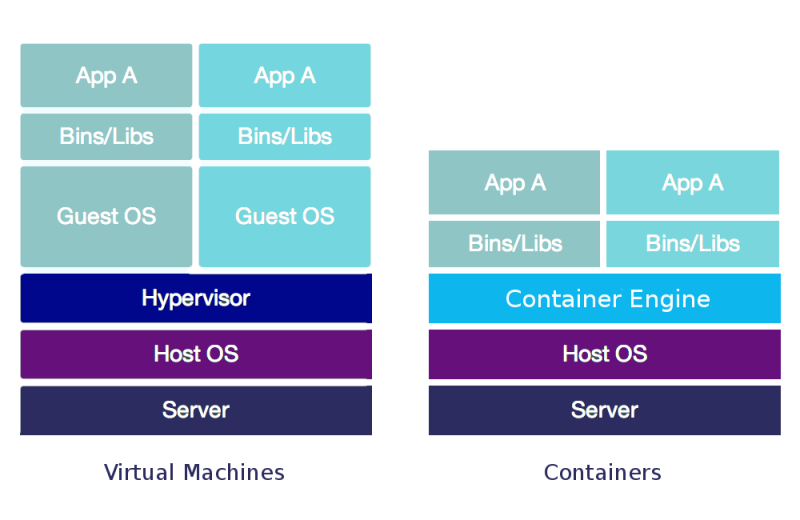
\includegraphics[width=0.6\textwidth]{images/docker_arch.png}
    \caption{Overview of a VM-based and container-based isolation architecture \cite{kumina}}
    \label{fig:container}
\end{figure}

Figure \ref{fig:container} shows the difference in computational overhead regarding traditional virtualization and container-based virtualization. The lightweight approach of containers enable the Host OS to support hundreds of containers on the same hardware.

Thus, containers can be viewed as a standard unit of software, a package which incorporates all the code and dependencies in a unit that can run on any computing system, in a quick and reliable manner.

\subsection{Docker}
Container images become containers at runtime and in the case of Docker containers - images become containers when they run on Docker Engine. Available for both Linux and Windows-based applications, containerized software will always run the same, regardless of the infrastructure. Docker container technology\cite{docker} was launched in 2013 as an open source container Engine. It leveraged existing computing concepts around containers and specifically in the Linux world, primitives known as cgroups and namespaces. The success in the Linux world drove a partnership with Microsoft that brought Docker containers and its functionality to Windows Server.

\subsection{Containers or Images, a clarification}
A container is launched by running an image. An image is an executable package that includes everything needed to run an application--the code, a runtime, libraries, environment variables, and configuration files. A container is a runtime instance of an image--what the image becomes in memory when executed (that is, an image with state, or a user process).

Images are built by the docker engine based on instructions that are written in a Dockerfile \cite{dockerfile} which defines what goes on in the environment inside the container. Access to resources like networking interfaces and disk drives is virtualized inside this environment, which is isolated from the rest of the system. For instance the user might need to instruct Docker to map certain ports from the container to the network interface of the host OS, or copy certain files from the host OS to the container (e.g configuration files, scripts, etc. ), an example is shown in Figure \ref{fig:dockerfile}.
\bigbreak
\noindent
\begin{figure}
\begin{minted}[%
 breaklines,
 mathescape,
 linenos,
 numbersep=5pt,
 frame=single,
 numbersep=5pt,
 xleftmargin=0pt
 ]{dockerfile}
    
# Use an official Python runtime as a parent image
FROM python:2.7-slim

# Set the working directory to /app
WORKDIR /app

# Copy the current directory contents into the container at /app
COPY . /app

# Install any needed packages specified in requirements.txt
RUN pip install --trusted-host pypi.python.org -r requirements.txt

# Make port 80 available to the world outside this container
EXPOSE 80

# Define environment variable
ENV NAME World

# Run app.py when the container launches
CMD ["python", "app.py"]
\end{minted}
\caption{A Dockerfile file example \cite{dockerfile}}
\label{fig:dockerfile}
\end{figure}

\subsection{docker-compose}
Docker compose (also called docker-compose)\cite{docker-compose} is a tool for designing and running multi-container applications. Following Docker‘s one application per container it is difficult to create or to containerize applications that have multiple components or servers. Thanks to docker-compose, the user can easily define multiple services (in a YAML file), link them together and run them. In the YAML file, the user defines each service as also the interdependence of the services. It informs docker on important attributes of each service, such as whether to use a container image from a registry or to build it locally with a Dockerfile. 

It also informs the docker engine on whether there are ports that are needed to be exposed (which can also be defined in a Dockerfile) as also on whether certain containers mush share file systems (using the volumes parameter) or if a service must wait for another before it starts. An example of a docker compose file can be seen in Figure \ref{fig:docker-compose} and further examination of the syntax can be found in the official documents\cite{docker-compose} of docker-compose.
\bigbreak
\begin{figure}[H]
\begin{minted}[%
 breaklines,
 mathescape,
 linenos,
 numbersep=5pt,
 frame=single,
 numbersep=5pt,
 xleftmargin=0pt
 ]{yaml}
version: '3'
services:
  web:
    build: .
    ports:
    - "5000:5000"
    volumes:
    - .:/code
    - logvolume01:/var/log
    links:
    - redis
  redis:
    image: redis
volumes:
  logvolume01: {}

\end{minted}
\caption{A docker-compose.yaml file example \cite{docker-compose}}
\label{fig:docker-compose}
\end{figure}

In conclusion, the Dockerfile defines a single microservice and it’s container, while the docker-compose defines the whole application and the relationships between the containers. There are container attributes that can be set from either file, the choice rests on various parameters of the application deployment.

Finally, Docker started an open-source project, Moby\cite{moby} to enable and accelerate software containerization. It provides a number of toolkit components and a framework for assembling them into custom container-based systems. Quite interestingly, our architecture is based on a project that is in turn based on Moby.


\subsection{Why Containers}

We opted to base our architecture on the containerization of microservices as it is in fact the foundation that makes our concept possible. Since containers are OS and hardware agnostic, the containerized microservices can run natively on any hardware, as long as it has the same CPU architecture (e.g RISC, x86, etc.) .
 
Thus, a service customer \textbf{SC} wishing to run some application logic on the service-provider’s \textbf{SP} Edge, simply: 1) packages the application into a number of clearly defined, stateless microservices, 2) agrees with the service-provider on the resources that \textbf{SP} will make available to the services and then 3) \textbf{SC} sends the container binaries to the \textbf{SP}.
 
It is important to note that the above mentioned 3-step functionality is complex and has many aspects that demand attention, from container management to security. \textit{The notion though rests unchanged.} 

\subsubsection{Container Security}

Security is an aspect that merits attentions, since containers are developed for use in trusted systems and not in multi-tenant environments as in the case of VMs. Containers offer a much more wide attack surface because the containers share the kernel linux. As such, critical bugs could result in malicious code being injected from one container to another or from one container to the hostOS ans vice-versa. Moreover, taken into account the network component of a multi-tenant container setup, containers or the hostOS could act as sniffers of the traffic passing through the same network bridge or even perform Man-in-the-Middle attacks. These kind of attacks can be mitigated by the use of a supervisor service which will monitor the activity of each container or by isolating the containers through multiple network bridges, but a thorough analysis is in order to verify feasibility.

Finally, we remind the user that all containers would run on the same hardware, giving extreme low-level attack surfaces to the IoT Edge owner since he will have physical access to the device.

\subsection{Balena}

For the system and fleet management of our IoT Edge Platform, we opted to choose balena\cite{balena}, a platform that is developed by balena.io, a Greek startup company that was founded in 2014, aiming to bring the docker container technology on IoT Edge devices, a non trivial task as docker container was developed with the needs of cloud computers at mind and not the unique needs and attributes of the relatively constrained IoT Edge devices (e.g Raspberry pi, Beaglebone, Intel Edison, etc.).

Balena offers a complete set of tools to manage and deploy fleets of connected Linux devices, i.e IoT Edge devices. Balena has many features, that we will mention in this subsection, but it’s pertinent to start with the one that interests us the most.

Balena has developed a bare-bones Yocto Linux based OS, named BalenaOS\cite{balenaos}, that can run on many common IoT Edge devices and architectures (e.g aarch64, armv7, etc.). In essence, to deploy applications on a balena powered device, the user deploys containers and manages them through the balena supervisor and balenaCloud\cite{balenacloud}. On top of that, balena has developed its own lightweight container technology, called balenaEngine\cite{balenaengine}, that is based on the Moby project and offers a docker compatible container technology that is \textit{superbly} optimised for the Edge.

\begin{figure}[h]
    \centering
    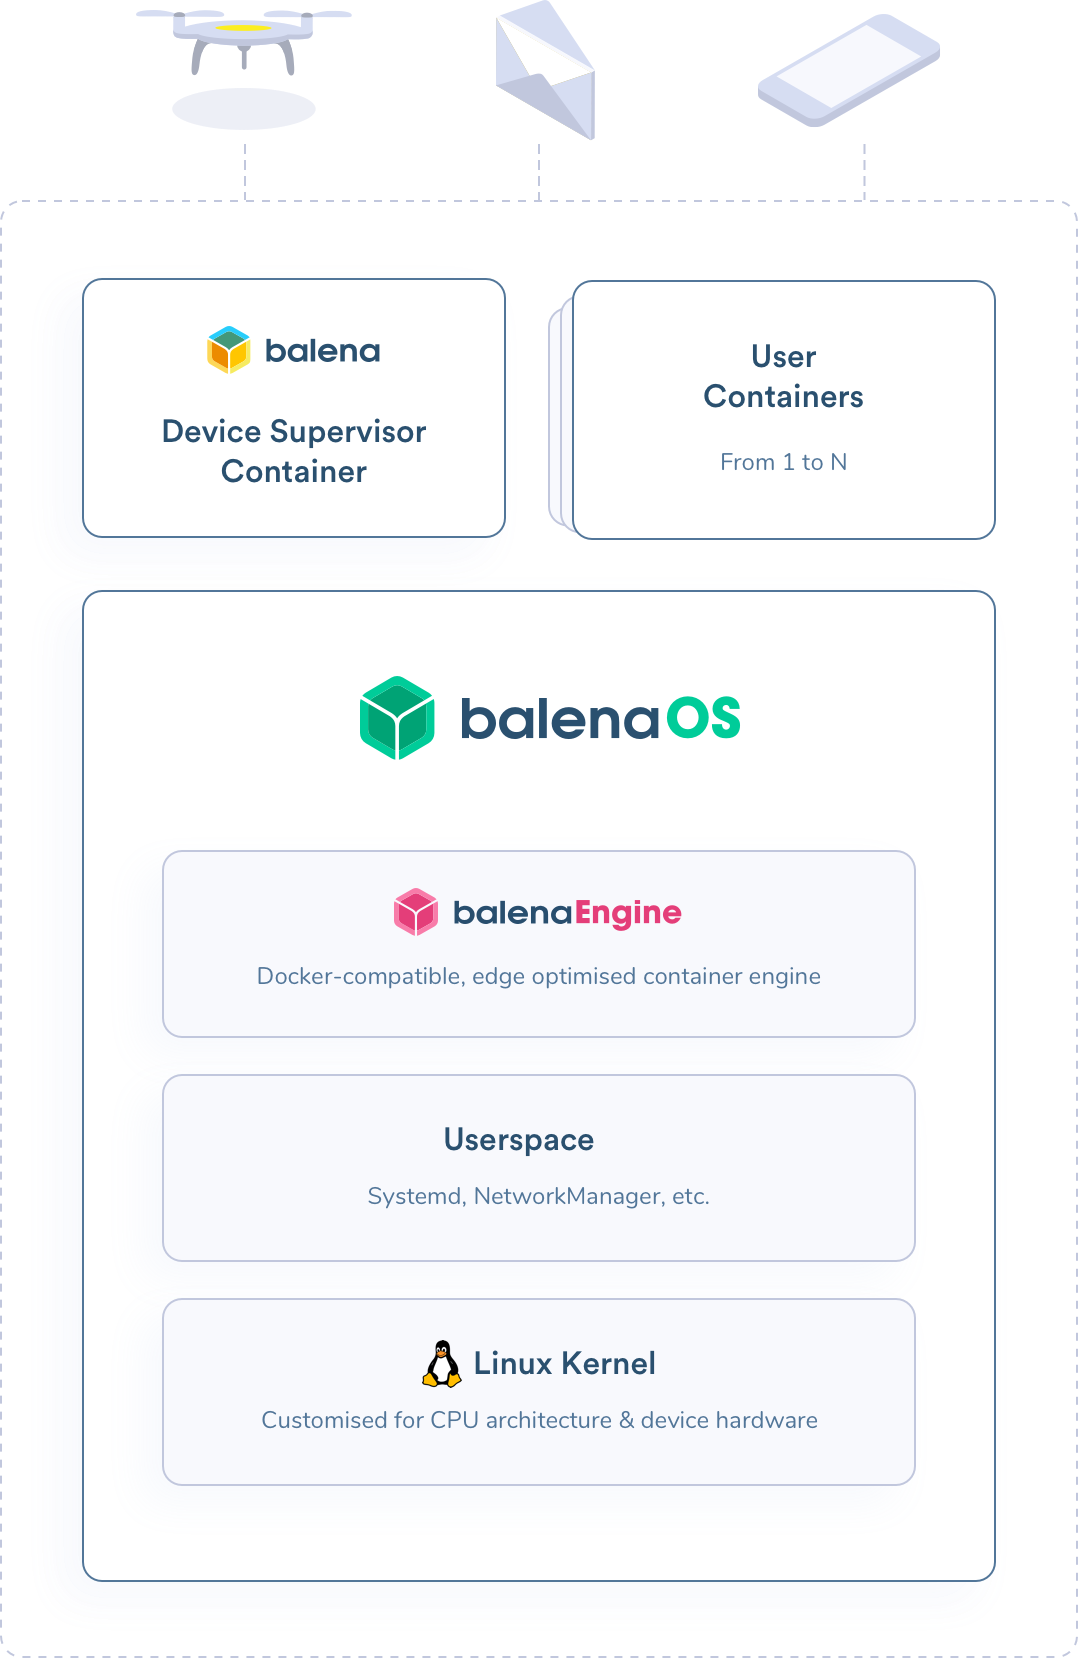
\includegraphics[width=0.5\textwidth]{images/balena_arch.png}
    \caption{The BalenaOS architecture \cite{balenaos}}
    \label{fig:balena_arch}
\end{figure}

\begin{figure}[h]
    \centering
    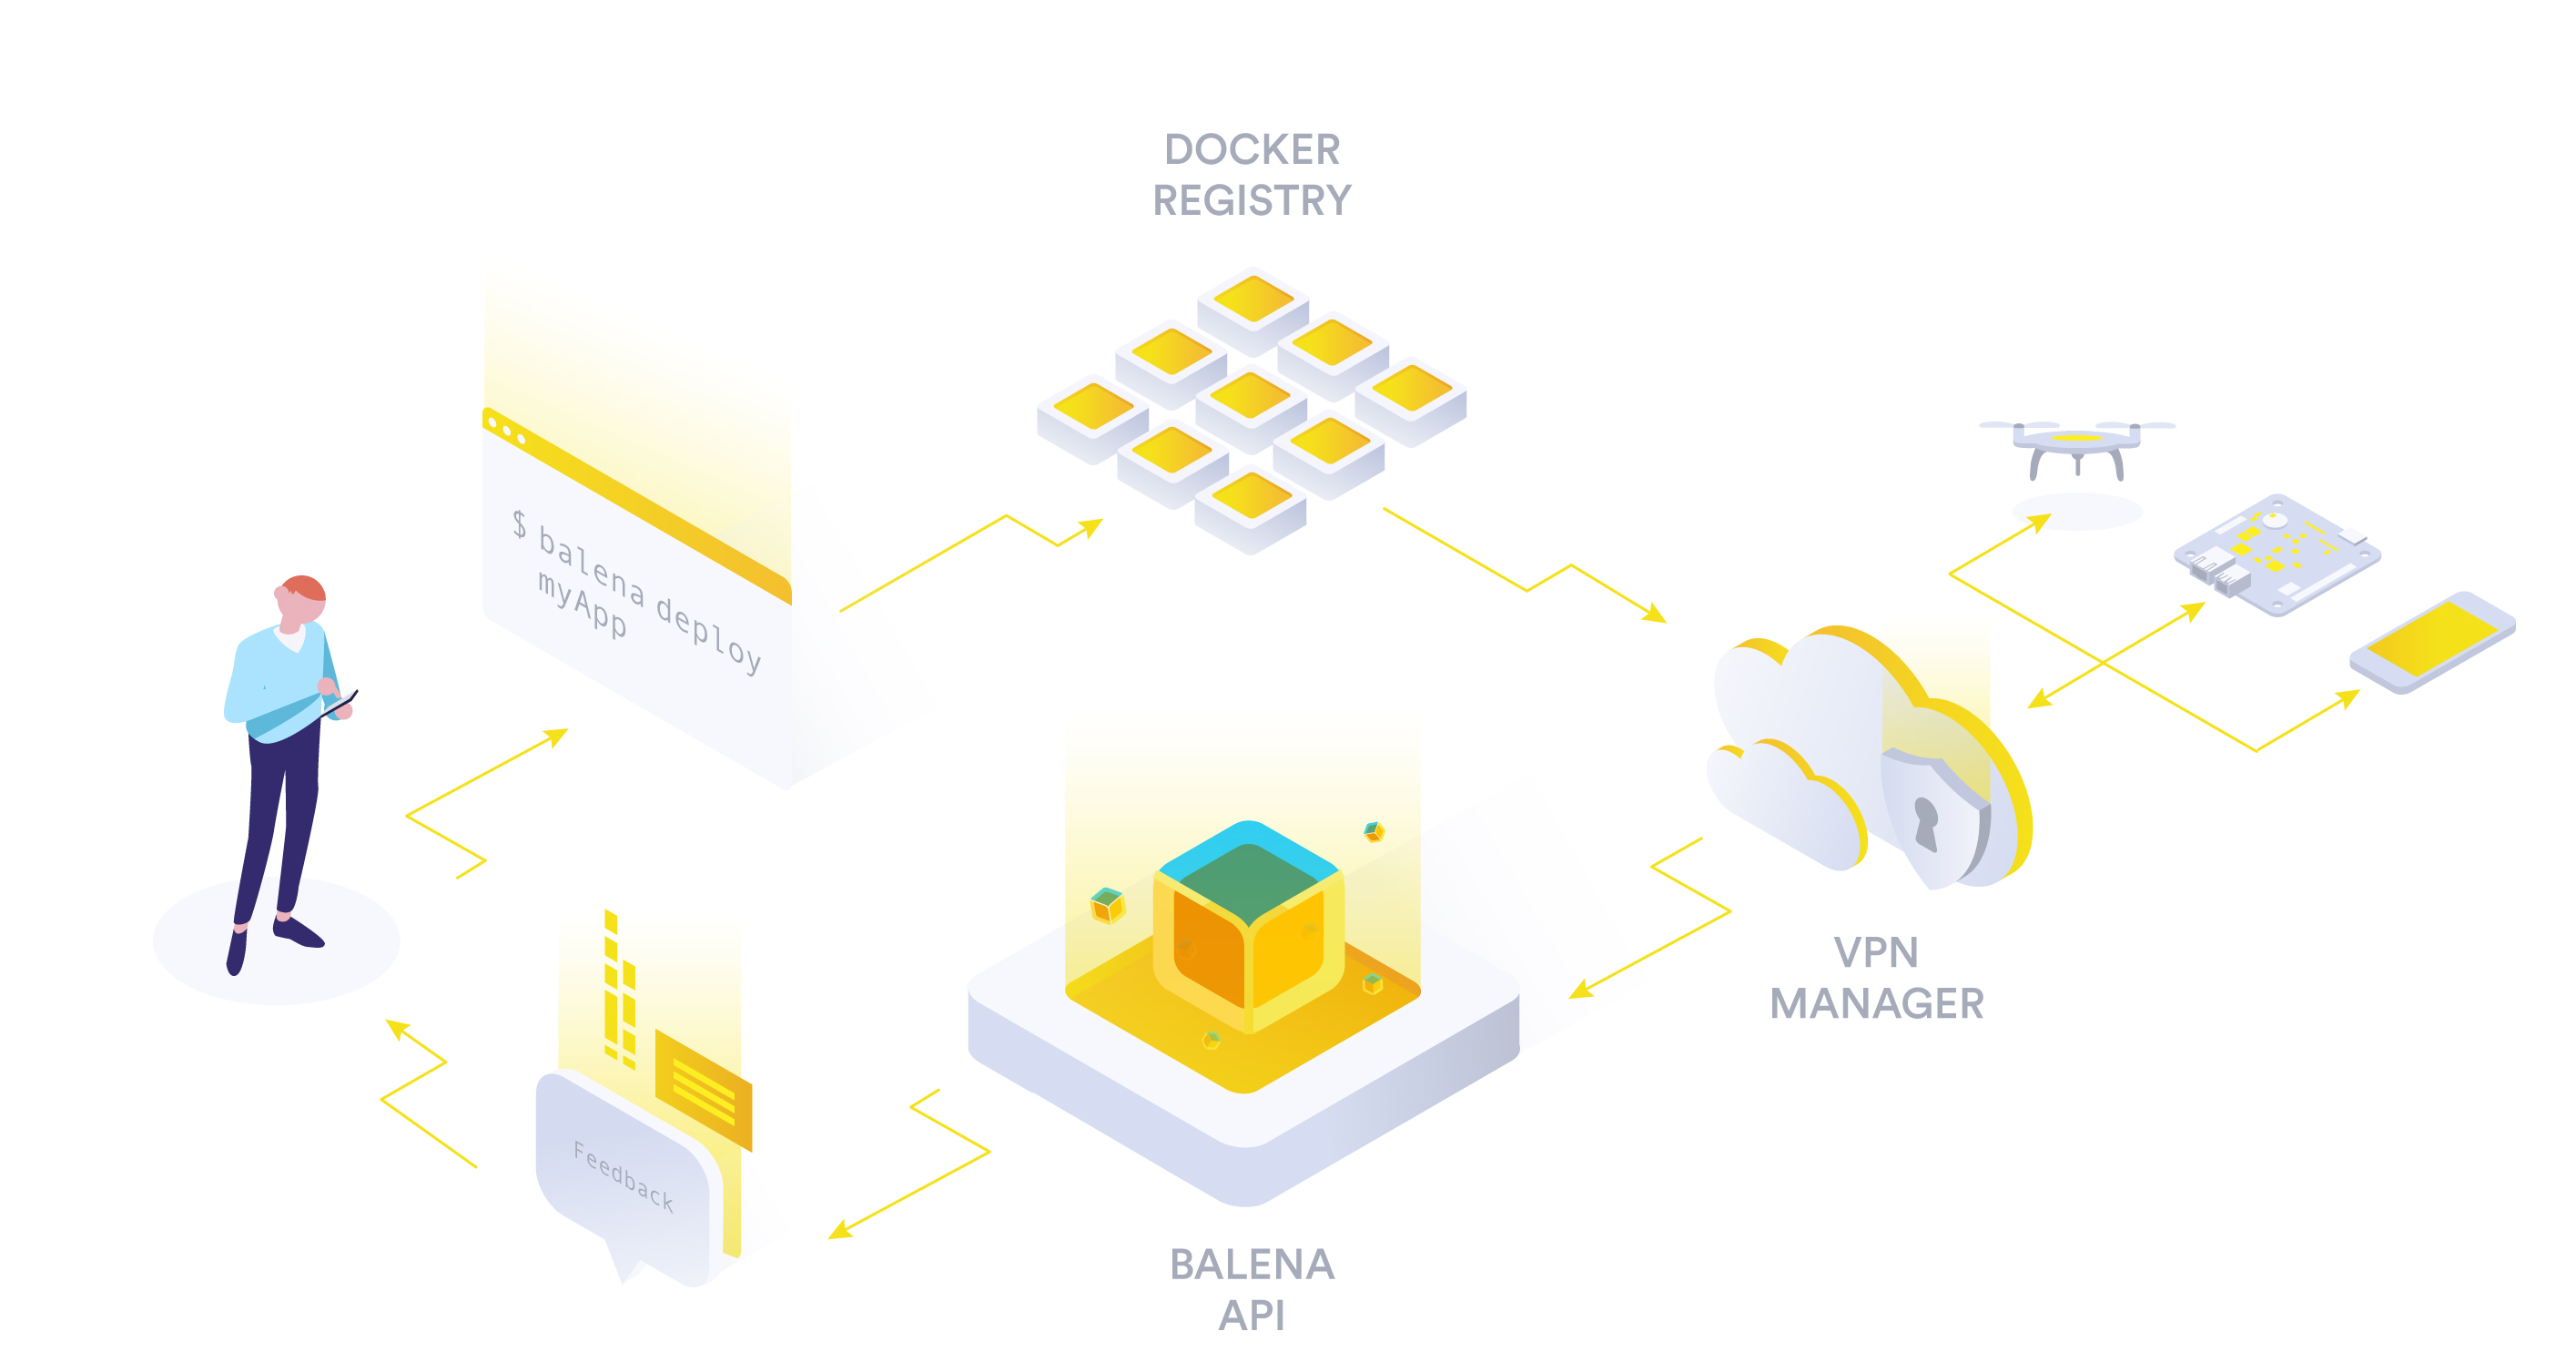
\includegraphics[width=0.9\textwidth]{images/balena_gen_arch.jpg}
    \caption{Overview of the Architecture of Balena Platform \cite{balena}}
    \label{fig:balena_gen_arch}
\end{figure}
\clearpage

Figure \ref{fig:balena_arch} outlines the main components of the balenaOS architecture. Note that the supervisor service rests in a containerized environment, ensuring that it will be able to manage the device and perform critical activities (e.g software update) even in the case of an application crash.

\subsection{Fleet Management using Balena}

The core balena platform, balenaCloud, encompasses device, server, and client-side software, all designed to get your code securely deployed to a fleet of devices. The general idea is that the developer creates an application and pushes it to balenaCloud, then the build servers package the application into containers and deliver them to the balenaOS devices. BalenaOS takes care of running, managing and monitoring the application, while balenaCloud offers on top a web interface to facilitate the fleet management. More in-detail information regarding the balena platform ecosystem can be found on their site\cite{balena}.

Figure \ref{fig:balena_gen_arch} illustrates the above mentioned architecture, where a user pushes the application's code to Builder, which builds it for the Device’s architecture and then ship ready container image binaries to each device.

\section{Decentralized Storage Solution} \label{st:filecoin}

\subsection{Filecoin Architecture} 

Filecoin is a decentralized storage network that turns cloud storage into an algorithmic market. The market runs on a blockchain with a native protocol token which miners earn by providing storage to clients. Conversely, clients spend Filecoin towards miners to store or distribute data (PUT) . The DSN scheme is a tuple of protocols run by storage providers and clients: (GET, PUT, MANAGE). The network architecture \& algorithms are described in the Filecoin White-paper \cite{filecoin-whitepaper}.
 
The Filecoin miners are divided into 2 types. \textbf{Storage Miners} who provide storage to the network (MANAGE) and Retrieval Miners that provide data retrieval to the Network. \textbf{Retrieval Miners} participate by serving data that users request ( GET ). It is natural for Storage Miners to also participate as Retrieval Miners. A high-level overview of how Filecoin works can be seen in Figure \ref{fig:filecoin}.

\begin{figure}[h]
    \centering
    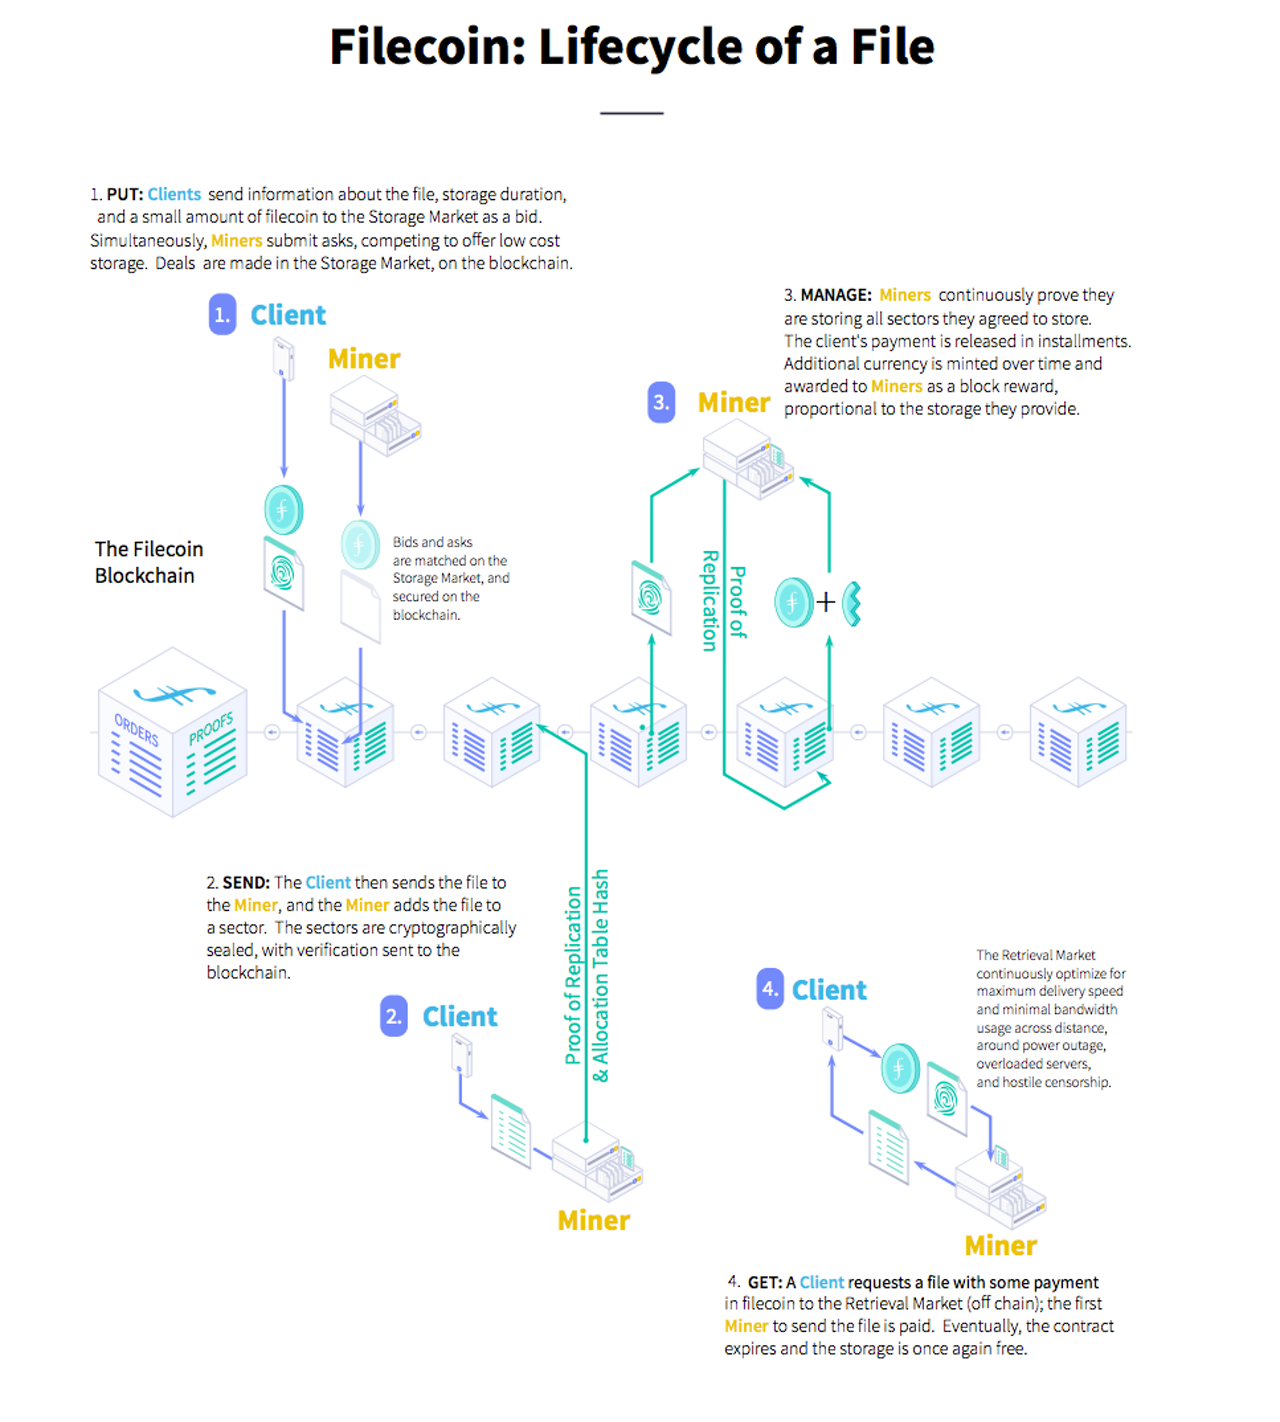
\includegraphics[width=1\textwidth]{images/filecoin.png}
    \caption{The filecoin high level architecture \cite{filecoin-primer}}
    \label{fig:filecoin}
\end{figure}
\clearpage

Filecoin works by creating two decentralized verifiable markets, the \textit{storage market} and the \textit{retrieval market}. Verifiable markets ensure that payment is paid when a specific service has been provided. Moreover, Filecoin introduces two proof-of-storage algorithms, which are used by the network nodes to reach consensus without wasting resources, as with the Proof of Work algorithm. The first algorithm is the proof-of-replication, which allows storage providers to prove that they have stored the data into distinct physical storages, while the second is the proof-of-spacetime algorithm and it allows them to prove that they store a piece of data for a specific amount of time. 

Currently, Filecoin is under heavy development and one could argue that the development progress is at pre-alpha stages, where the foundation is being laid and the protocols are implemented so as Filecoin works in a prototype manner. The markets do not currently function as a dynamic and automated market, but rather in a manual fashion, where a client selects a storage provider from an ask-list and the commits a file to be saved. The storage provider accepts any deal that is proposed from a storage client and matches an ask deal that he has made, regardless the storage it requires. Finally, the network works with devnet FIL that are used for testing purposes and will be reset when the network comes online.

Thus, the proposed Back-End Node participate in the network as both Retrieval \& Storage Miner. By serving as both, it can save locally the data sent by the Edges to the DSN for faster access times. Meanwhile, in Filecoin the data are expected to be saved in multiple locations, providing the necessary data integrity layer that we want. Finally, by participating in the network, the stakeholder’s Cloud will “earn” Filecoin (FIL) that can be used to finance the use of the DSN by the stakeholder’s Edges. Note that Filecoin is expected to have “smart contracts” functionality in the future, enabling thus the system to save for free the data in its own cloud while paying only for the extra copies in other storage providers.

\subsection{Blockchain}

The blockchain is considered to be one of the most groundbreaking innovations of the last decade, foreseeing a completely decentralized future where consensus and \gls{trust} are built upon mathematical models. It is essentially a distributed database of records of transactions - a ledger - where all the nodes in the network participate actively to reach a consensus on the final status of the database. Figure \ref{fig:blockchain} showcases a database which is structured as a chain of blocks, where each block references the last one and encapsulates a number of transactions (database records).  The Merklee Root is the root of Merklee tree (tree of hashes) which can be seen as a succinct proof of the existence of N different elements, in our case transactions. Once a block has been appended to the data structure (ledger), it is impossible to remove or alter it (due to the reference mentioned above). The notion of blockchain  was introduced in 2008 by Satoshi Nakamoto\cite{bitcoin}. It uses well known cryptographic systems, such as public key cryptography\cite{pubkey} and \acrfull{pow}\cite{bitcoin} to create a system where value can be transferred without the need for intermediaries. Bitcoin was the first open source project to implement this new vertical which created the notion of cryptocurrencies. PoW is a process where a computer solves a cryptographic puzzle and is used in various projects, most prominently bitcoin, as a consensus mechanism.

\begin{figure}[h]
    \centering
    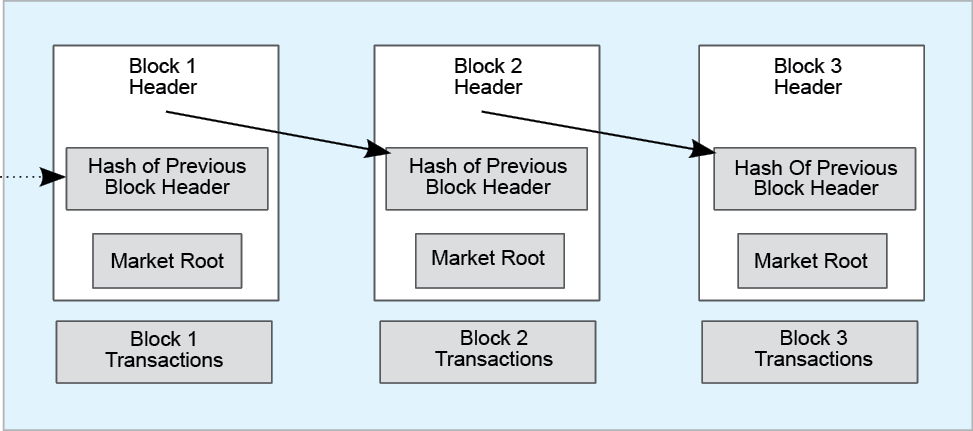
\includegraphics[width=0.6\textwidth]{images/blockchain.jpg}
    \caption{A reference blockchain architecture\cite{opensourceforu}}
    \label{fig:blockchain}
\end{figure}

Finally, blockchain are characterized by 2 important attributes, \gls{permission} and trust. The technology was popularised from projects, such as the bitcoin, explicitly for being permissionless and trustless

\section{Container Migration on balena using Filecoin} \label{st:balena-filecoin}

In the proposed architecture, the “IoT Edge as a service” functionality is provided by running strictly defined services over a pre-agreed amount of IoT Edge device resources. In order to strictly define the resources, the use of docker technology is chosen, containers, in other words, that are acknowledged as units of software that are stateless and atomic (without dependencies). The service customer procures to the service provider a set of containers that will be run when the service contract is activated, at a pre-configured event (or even immediately).

\subsection{Service customer}

For the migration to adhere to the principles of data integrity and high availability, the image containers are stored in the Filecoin Network, always accessible using a unique key, called \textit{CID} in Filecoin and image\_hash in our implementation. The service customer is responsible for ensuring the existence and functionality of the images stored in the network.

In the current version of Filecoin, a file stored in the network can be retrieved  using the file \textit{CID} and the ID of the storage provider with whom the storage deal was made. Thus, each stored file $F$ is characterised by the following tuple $S_f = [CID, miner\_ID]$ and the Service Customer must send a $S_f$ to the Service Provider for each file $F$ that is stored in the network.

\subsection{Service Provider}

The service provider uses the procured CID to request from the Filecoin DSN the files and download them. It downloads a set of containers and a set of corresponding configuration files.

\begin{enumerate}
    \item The images are loaded into balenaEngine using HTTP request to a unix socket that is exposed in the orchestrator container from the balena HostOS. 
    \item The orchestrator uses the supervisor’s API to GET the state of the device’s application. This state is a considerably large data structure in JSON format which describes the entirety of the device, from low-level aspects towards what services run and with what  
    configurations. 
    \item The orchestrator constructs the descriptions of the service customer’s containers according to the schematic of the balena supervisor’s API and the configuration file of each container. As the reader might suspect, each container will use an image that was just loaded to balenaEngine in step (1).
    \item The orchestrator makes a POST request to the supervisor’s API with the device’s state that was GET in step (2), modified to include the service’s state that was generated in step (3).
\end{enumerate}

The above described migration processes is outlined in two distinct Algorithms \ref{alg:algorithm1} and \ref{alg:algorithm2}, from the perspective of service customer (who initiates the process) and the service provider (who finishes the process).

\subsection{Development OS and Local Mode}
The above can only be implemented, with a current version of balenaOS and balenaCloud (or openBalena), if the device uses a development version OS and is configured to work on local mode\cite{localmode}. This is highly important, because a development OS local mode device can manually load images into BalenaEngine and push new releases locally, without the need of BalenaCloud(i.e manually setting the device's \textit{state} using the supervisor API). Having said that, development OS facilitates the development and debugging but exposes the device to serious security risks can \textbf{should not be used in production environments}. Thus, we have concluded that a production ready platform would need to build on top of balenaOS from scratch, with heavy modifications on the supervisor, both of which are open sourced.

\subsection{A centralized interim solution \textit{(perhaps)}}

With the above solution, we strived for the autonomy of the IoT Edge device, having zero dependencies when functioning as a service provider, especially when providing a fault-tolerance insurance.

But, it is possible to simplify the above process, by using a back-end cloud system where Balena-CLI is installed. Then, using a simple web application that will function as a simple HTTP RESTful API for the Balena-CLI, we could follow the following approach:

\begin{enumerate}
    \item Instead of downloading the images locally, instruct the backend to download the service customer’s images from the filecoin DSN.
    \item GET the docker-compose.yaml file from the BackEnd.
    \item Append the service customer’s service into the docker-compose.yaml file downloaded in step (2), according to the specifications found in the configuration file.
    \item Make a POST request to the back-end and upload the new docker-compose.yaml.
    \item Instruct the backend to run the command “\texttt{balena push <application\_name>}".
\end{enumerate}

The configuration files describe the settings that are needed for the containers to function properly (e.g exposed ports). Currently,  the configuration file also dictates the contract activation clauses, indicating to the orchestrator when the services will need to start, as well as the Filecoin storage provider(miner) ID. The contract clauses are expected to exist in a separate contract data structure which also will define the system resources that will be provisioned for the services. An example of the configuration file can be found in Figure \ref{fig:configuration-file}.

\begin{figure}
\centering
\begin{minted}[%
 breaklines,
 mathescape,
 linenos,
 numbersep=5pt,
 frame=single,
 numbersep=5pt,
 xleftmargin=0pt
 ]{json}
    {
    "service_customer_id":"EdgeX-64",
    "serviceName": "nodered-device-service",
    "activationEvent": "offline",
    "event":{
        "interval": "20",
        "ip":"https://f223871f69c8b68a509868943f84bf7b.balena-devices.com/"
    },
    "ports": "1880",
    "volumes": "node-red-data:/data",
    "depends_on":["lora-appserver","edgex-core-command", "edgex-core-data","edgex-core-consul","orchestrator"],
    "miner_address": "t1hieq4dc3y3tlptg3xy2nb4ruczlomcixak2we4a"
}
\end{minted}
\caption{Reference structure of the configuration.json file}
\label{fig:configuration-file}
\end{figure}

\begin{algorithm}
% \begin{algorithmic}[1]
Build container image $C_j$ from Dockerfile\;
Create configuration.json  $Y_j$ \;
Upload container image $C_j$ to Filecoin DSN\;
   $X_j$  $\leftarrow$ container image File CID \;
Upload configuration file $Y_j$ to Filecoin DSN\;
   $Y_j$ $\leftarrow$ configuration file CID \;
Send $X_j$ to Service Provider\;
Send $Y_j$ to Service Provider\;
% \end{algorithmic}
\caption{Algorithm  1 Migration - Preparation. Actor: Service Customer}
\label{alg:algorithm1}
\end{algorithm}

\begin{algorithm}

Download image $I_j$ from Filecoin DSN using $X_j$ \;
Download configuration file $C_j$  from Filecoin DSN using $Y_j$ \;
configuration $\leftarrow$ $C_j$ \;
event\_type $\leftarrow$ configuration.event\_type  \;
event\_conditions $\leftarrow$ configuration.event\_conditions \;
service\_name $\leftarrow$ configuration.service\_name \;
Load $I_j$ $\rightarrow$  balenaEngine \;
Set supervisor state \;
\While {contract is active}{
    event $\leftarrow$ current event\;
    \eIf {event is in contract\_event and event\_conditions are true}{
        Start service (service\_name input) \;
        Break \;
    }{
    Continue \;
    }
}
\caption{Algorithm 2 Migration. Actor: Service Provider}
\label{alg:algorithm2}
\end{algorithm}
\clearpage

\begin{sidewaysfigure}
    \centering
    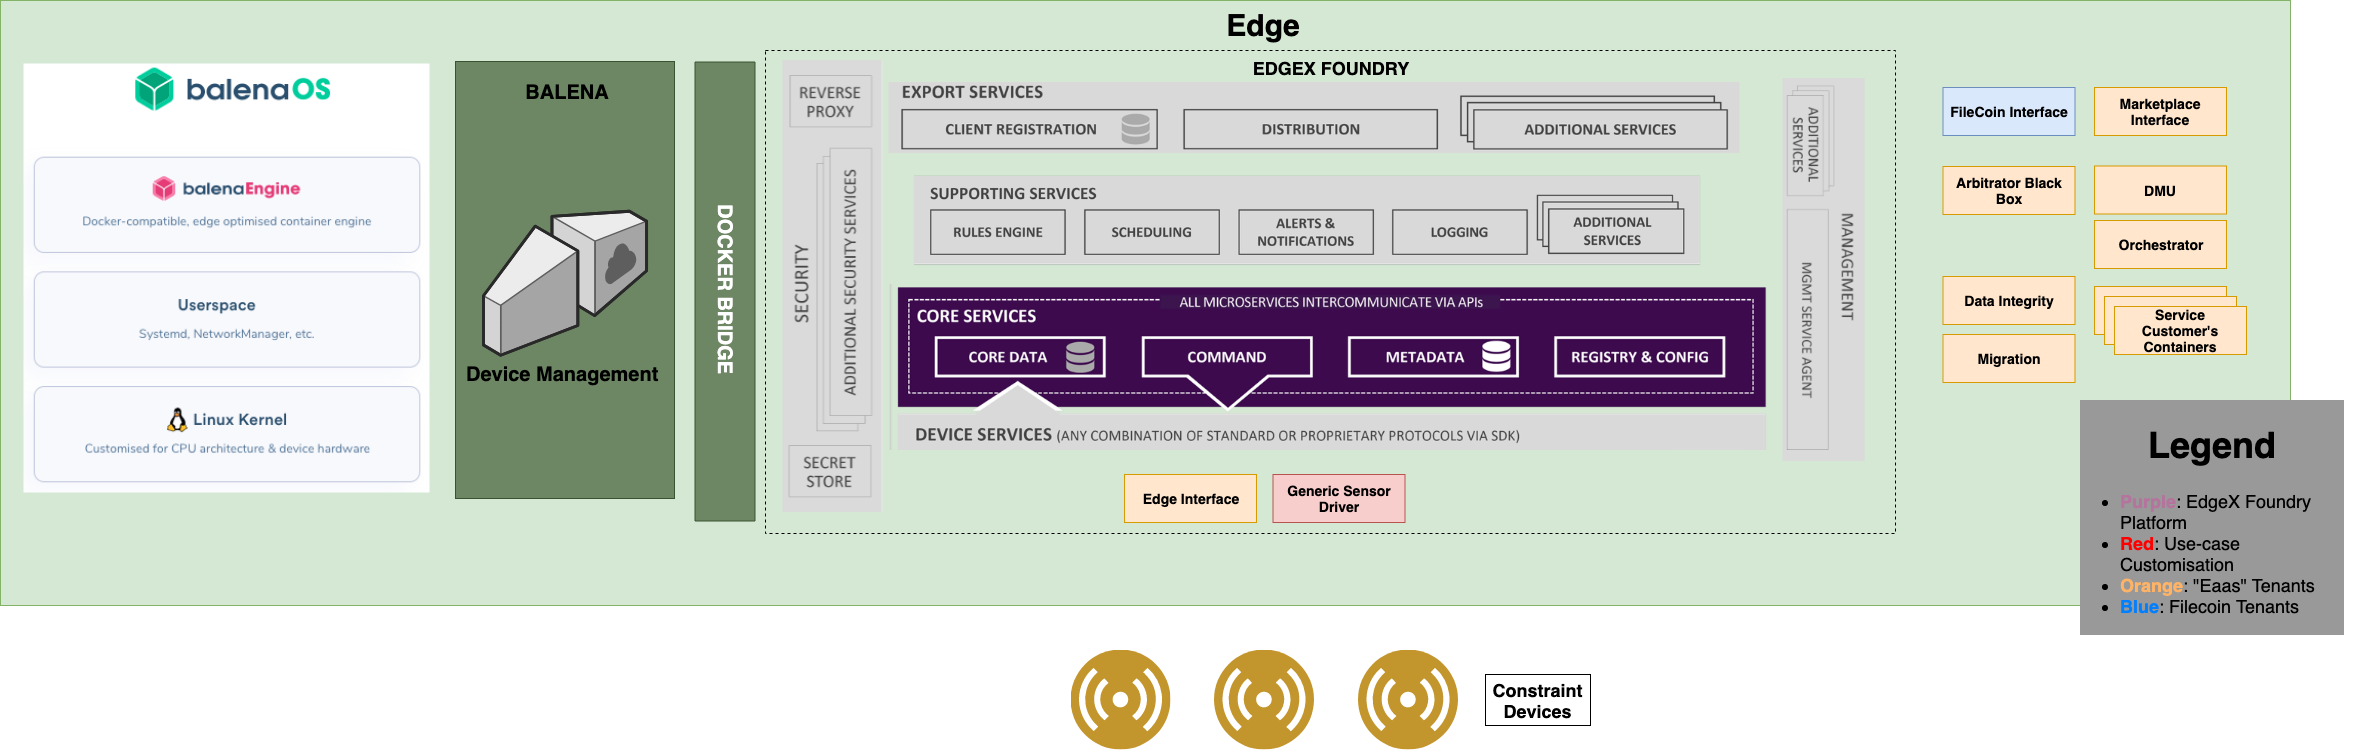
\includegraphics[width=1\textwidth]{images/EdgeArch_v7.png}
    \caption{The high level proposed architecture of an IoT Edge device}
    \label{fig:edge}
\end{sidewaysfigure}

\section{IoT Edge Architecture}

The IoT Edge can have different forms depending on the IoT application needs, ranging from a micro-computer with industry standards, to even a micro Data Center to support computational demanding localised AI services. Although the number of IoT Edge devices and their computational power can differ considerably, our architectural approach is relevant without altering the core functionality and the unique features that we envisage to support.
 
In order to create a highly modular and robust system, we turned to the microservices paradigm adjusted for the needs and abilities of the Edge. Following the principle of loosely-coupled services, each service is placed in its own container, even those belonging to the same platform (e.g EdgeX Foundry). The containers communicate through HTTP REST calls using Docker Bridges and each container will be configured appropriately for the service it hosts. As such, services that handle hardware or need Internet Access will have more \textit{“access control rights”} than other services. An overview of the architecture is shown in Figure \ref{fig:edge}.

\subsection{IoT Edge Architecture reference services}
\begin{enumerate}
    \item \textbf{"IoT Edge as a service” Modules}
    \begin{enumerate}[label*=\arabic*.]
        \item \textbf{DMU:} This service is responsible for evaluating the contracts in the IoT Edge Marketplace. Whether concerning an offer or the parameters of a demand. The simplest form is rule-based.
        \item \textbf{Arbitrator:} The service that is responsible for ensuring that every party in an service contract act as a trusted party.
        \item \textbf{Migration:} The service responsible for uploading \& downloading the necessary images in the DSN.
        \item \textbf{Edge2Edge Interface:} The service is responsible for inter-Edge communication.
        \item \textbf{Orchestrator:} Responsible for managing and overseeing the service provision process.
        \item \textbf{Marketplace Interface:} A Restful API that is responsible for probing the marketplace and fetching information from it (i.e offers).
        \item \textbf{Service Customer Containers:} All the containerized services of the service customer that remain idle until their activation by the orchestrator.
        \end{enumerate}
    \item \textbf{Filecoin Modules:}
        \begin{enumerate}[label*=\arabic*.]
        \item \textbf{Filecoin Interface:}  This service is responsible for connecting with the Filecoin network, uploading \& downloading the necessary content.
        \end{enumerate}
\end{enumerate}

\subsection{IoT Edge Platform}

Our approach for the IoT Edge is to expand an existing solution with services that will enable it to offer the envisaged functionalities of our proposal. The main platform chosen to be responsible for performing much of the usual IoT Edge functionality, as already mentioned, is EdgeX Foundry.

\subsection{Device Management at the Edge}

The role of device management is realised by Balena. The host OS is responsible for kicking off the device supervisor, balena’s agent on a device, as well as our containerized services. Within each service's container we can specify a base OS, which can come from any existing Docker base image that is compatible with our device architecture.  

\subsection{Data Integrity at the Edge}

Data Integrity is considered a key aspect of the proposed design. It ensures the overall completeness, accuracy and consistency of data. This can be indicated by the absence of alteration between two instances or between two updates of a data record, meaning data is intact and unchanged.
 
Data Integrity will be enforced from end-to-end, from the IoT Edge that aggregates sensor data to the cloud that serves them. We consider a scheme where each IoT Edge has a unique private key generated at a setup phase, unknown to the centralized Cloud Back-End, that is used as a unique device signature.
 
As per the Edgex architecture, the data integrity service will receive the sensor data from the distribution service in the export services layer. The service then will create a certain proof (e.g. hashing) of a certain unit of data. This proof will be publicly accessible and auditable, say by publishing it in a blockchain or storing in it Filecoin and publicly announcing the key to retrieve it. Thus, if the integrity of the data is requested, the cross-checking of the proof and the data themselves will provide the necessary integrity. 

We feel that there is no need to strictly define the integrity module as it attributes can change depending on the use-case of the IoT Edge device. Critical infrastructure could demand a more thorough and secure fashion, which impedes ease of use and efficiency but more common applications could opt for a better user-experience.
 
One could argue that the data integrity process should be embedded in the core data service, which functions as a centralized gateway for all sensor data in the Edgex platform, but we estimate that we can implement it as an add-on. This is due to the fact that Edgex services are considered as tamper-proof from the user, thus trusted. As they are trusted, they will function as we expect them to and as a result, they will  certainly propagate the data to the data integrity add-on service to construct the proof.
 
On top of that, Filecoin ensures that the data will securely be stored in multiple physical storage locations and thus will not have a single point of failure. In each Edge, the Filecoin Interface Module will package the data needed to be delivered and will make a bid order in the Filecoin Storage Market. The IoT Edge will provide to the Cloud Back-End the necessary keys in order to access the data in the DSN for various purposes (i.g analytics, history, etc. ).  

Finally, we underline that the IoT Edge device owner must be able to finance the use of the Filecoin network, either buying FIL in the market (i.e through exchanges) or using his Cloud Back-End as Filecoin miner. The exact economics and cost analysis are outside the scope of the Thesis and impossible to determine, as the Filecoin network hasn’t launched as of September 2019.
 
\subsection{Fault-Tolerance}

At specific arbitrary occasions, the IoT Edge will begin the process in order to find another IoT Edge device that will serve as the insurance provider. The insurance provider will not only hand-over the devices of the IoT Edge but will also perform any pre-processing or other arbitrary activity. 

The Nodes (IoT Edge Devices) can participate in a centralized IoT Edge Market where Stakeholders can find service-providers or offer their cloud as a Sibling. A service-provider (or more specifically, insurance-provider) is an IoT Edge that has made a specific contract with another IoT Edge to serve as a backup server in case of critical failure. Although the offered services can vary, the main responsibilities are expected to be: 1)Constrained devices handover 2) Data preprocessing 3) North-side data forwarding.

The IoT Edge Market is a centralized service offered by the system’s manufacturer or a IoT Edge federation. It offers the possibility for cloud to find available IoT Edge and then negotiate directly. The Decision Making Unit (DMU) reviews offers, either as customer or provider, and decide on their prospect. If agreement is reached, the central system is informed and the IoT Edge Arbitrators create the contract and inform the central arbitrator authority.
 
Fault-Tolerance is presented in detail in the Section \ref{st:fault-tolerance} .

\section{Cloud Layer Architecture}

While neither the implementation, nor the architecture focuses on the cloud layer architecture, we believe that it is worth giving the general gist of the architecture, in order to outline the holistic approach of our architecture regarding both layers (Edge, Cloud).

\begin{figure}[h]
    \centering
    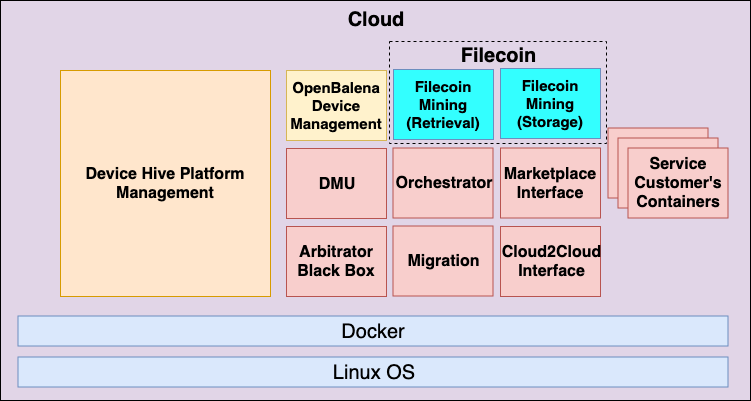
\includegraphics[width=0.9\textwidth]{images/CloudArch_v6.png}
    \caption{High level overview architecture of a Cloud system}
    \label{fig:cloud}
\end{figure}

The system generally follows the paradigm of an IoT platform, using a central Back-End to orchestrate various IoT Edge devices, aggregate data, perform heavy computations, analytics and offer interfaces for 3rd party services or for the system admin. The Cloud Module belongs to a larger network of Cloud Nodes that participate in a service marketplace offering or demanding the computational resources, much like in the IoT Edge architecture .Thus, we can consider the Cloud Module as a Back-End Node in a Graph of relatively homogeneous (software-wise) Systems.
 
The architecture is agnostic on the specific hardware or cloud solution, but we project common infrastructure in a linux server distribution, such as Ubuntu or Debian. The architecture follows the microservices paradigm and the intercommunication is done using Docker bridges and the HTTP protocol (RESTful APIs). The necessary infrastructure for the various services (such as registry, message bus, etc.) is offered by the reference core platform, DeviceHive\cite{devicehive}. The architecture is shown in Figure \ref{fig:cloud}.

\subsection{Cloud Architecture reference services}

\begin{enumerate}
    \item \textbf{"IoT Edge as a service” Modules:}
    \begin{enumerate}[label*=\arabic*.]
    \item \textbf{DMU:} This service is responsible for evaluating the contracts in the Cloud Marketplace, whether concerning an offer or the parameters of a demand. The simplest form is rule-based.
    \item \textbf{Arbitrator:} The service that is responsible for ensuring that every party in an insurance contract is a trusted party.
    \item \textbf{Migration:} The service responsible for uploading \& downloading the necessary images in the DSN.
    \item \textbf{Cloud2Cloud Interface:} The service is responsible for inter-cloud communication.
    \item \textbf{Orchestrator:} Responsible for managing and overseeing the service provision process.
    \item \textbf{Marketplace Interface:} A Restful API that is responsible for probing the marketplace and fetching information from it, such as offers.
    \item \textbf{Service Customer Containers:} All the containerized services of the service customer remain idle until being activated by the orchestrator.
    \end{enumerate}
    \item \textbf{Filecoin Modules:}
     \begin{enumerate}[label*=\arabic*.]
     \item \textbf{Filecoin Interface:}  This service is responsible for connecting with the Filecoin network, uploading \& downloading the necessary content.
    \end{enumerate}
    \item \textbf{IoT Edge Platform Management \& Device Management services}
 \end{enumerate}  

\subsection{IoT Edge Platform Management}
    The IoT Edge Platform Management is responsible for aggregating the data from the IoT Edge devices (uplink), issuing (downlink) commands relevant to their functionality (e.g. activating an actuator, etc.) and offering services (e.g. analytics) to users and 3rd party services. Moreover, the IoT Edge Platform Management provides the necessary infrastructure (e.g message bus), for all the cloud Modules to communicate with other Modules or Systems.
    
    There are numerous platform management solutions coupled with production ready infrastructure and services, such as Google IoT, AWS IoT Core, Microsoft Azure, etc. We have focused our research on Open Source Solutions that are characterized by maturity, vibrant community as also modularity. The platform of choice to use as a reference is DeviceHive, as it offers unique modularity and is structured as an array of containerized microservices. Device Hive also serves as a proxy with the south side (Edge) using a multitude of available protocols (HTTP REST, MQTT, CoAp, etc.).
    
\subsection{Fleet Management}
As described in the IoT Edge section, the fleet management solution is Balena, but instead of using the payed service provided by Balena.io, we will be using the Open Source solution OpenBalena that will be hosted in the Back-End Node. The service is responsible for offering the Balena Dashboard, building and serving the container images to the Edges, provisioning new IoT Edge devices and performing OTA (Over-the-Air) updates.

\subsection{Platform Management vs Device Management}
We consider platform management as the process of managing the various functionalities and services of the IoT Edge devices, such as aggregating data, performing analytics, controlling actuators, etc. Fleet management is the process of managing the IoT Edge themselves, provisioning new devices, performing Updates Over Air (OTA), maintenance, etc.

\subsection{Fault-Tolerance}
The structure of the Fault-Tolerant group of Modules is similar to the Edge’s. The Nodes (Cloud modules) can participate in a centralized Cloud Market where Stakeholders can find service-provider s or offer their cloud as a Sibling. A service-provider is a cloud that has made a specific contract with another cloud to serve as a backup server in case of critical failure. Although the offered services can vary, the main responsibilities are expected to be: 1)IoT Edge systems hand-over 2)data processing 3)API for 3rd party services and many more custom tailored services.
 
The Cloud Market is a centralized service offered by the system’s manufacturer or a cloud federation. It offers the possibility to the cloud to find available service-providers and then negotiate directly. The service-provider Decision Making Unit (DMU) reviews offers, either as customer or provider, and decide on their prospect. If agreement is reached, the central system is informed and the Arbitrators create the contract and inform the central arbitrator authority.
 
Fault-Tolerance is presented in detail in the Section \ref{st:fault-tolerance}.

\section{Sensor Layer}
The proposed architecture exploits the unique features of Edgex, namely its extreme modularity and customizability. As mentioned above, the containerized microservices architecture enables both the system provider and the stakeholder to equip the IoT Edge Node with literally any sensor or constraint device that the hardware can support. As such, we are completely agnostic in regards to the nature of the sensor as long as the device service that handles that particular sensor follows the Edgex specifications.

It is pertinent to mention that the Sensor Layer is prone to cyber and physical attacks, both because of easy physical access (usually) and because of low processing power which results in limited cryptographic functionalities. Nonetheless, our architecture is Sensor Layer agnostic and thus such an analysis falls outside of the scope.

\begin{sidewaysfigure}
    \centering
    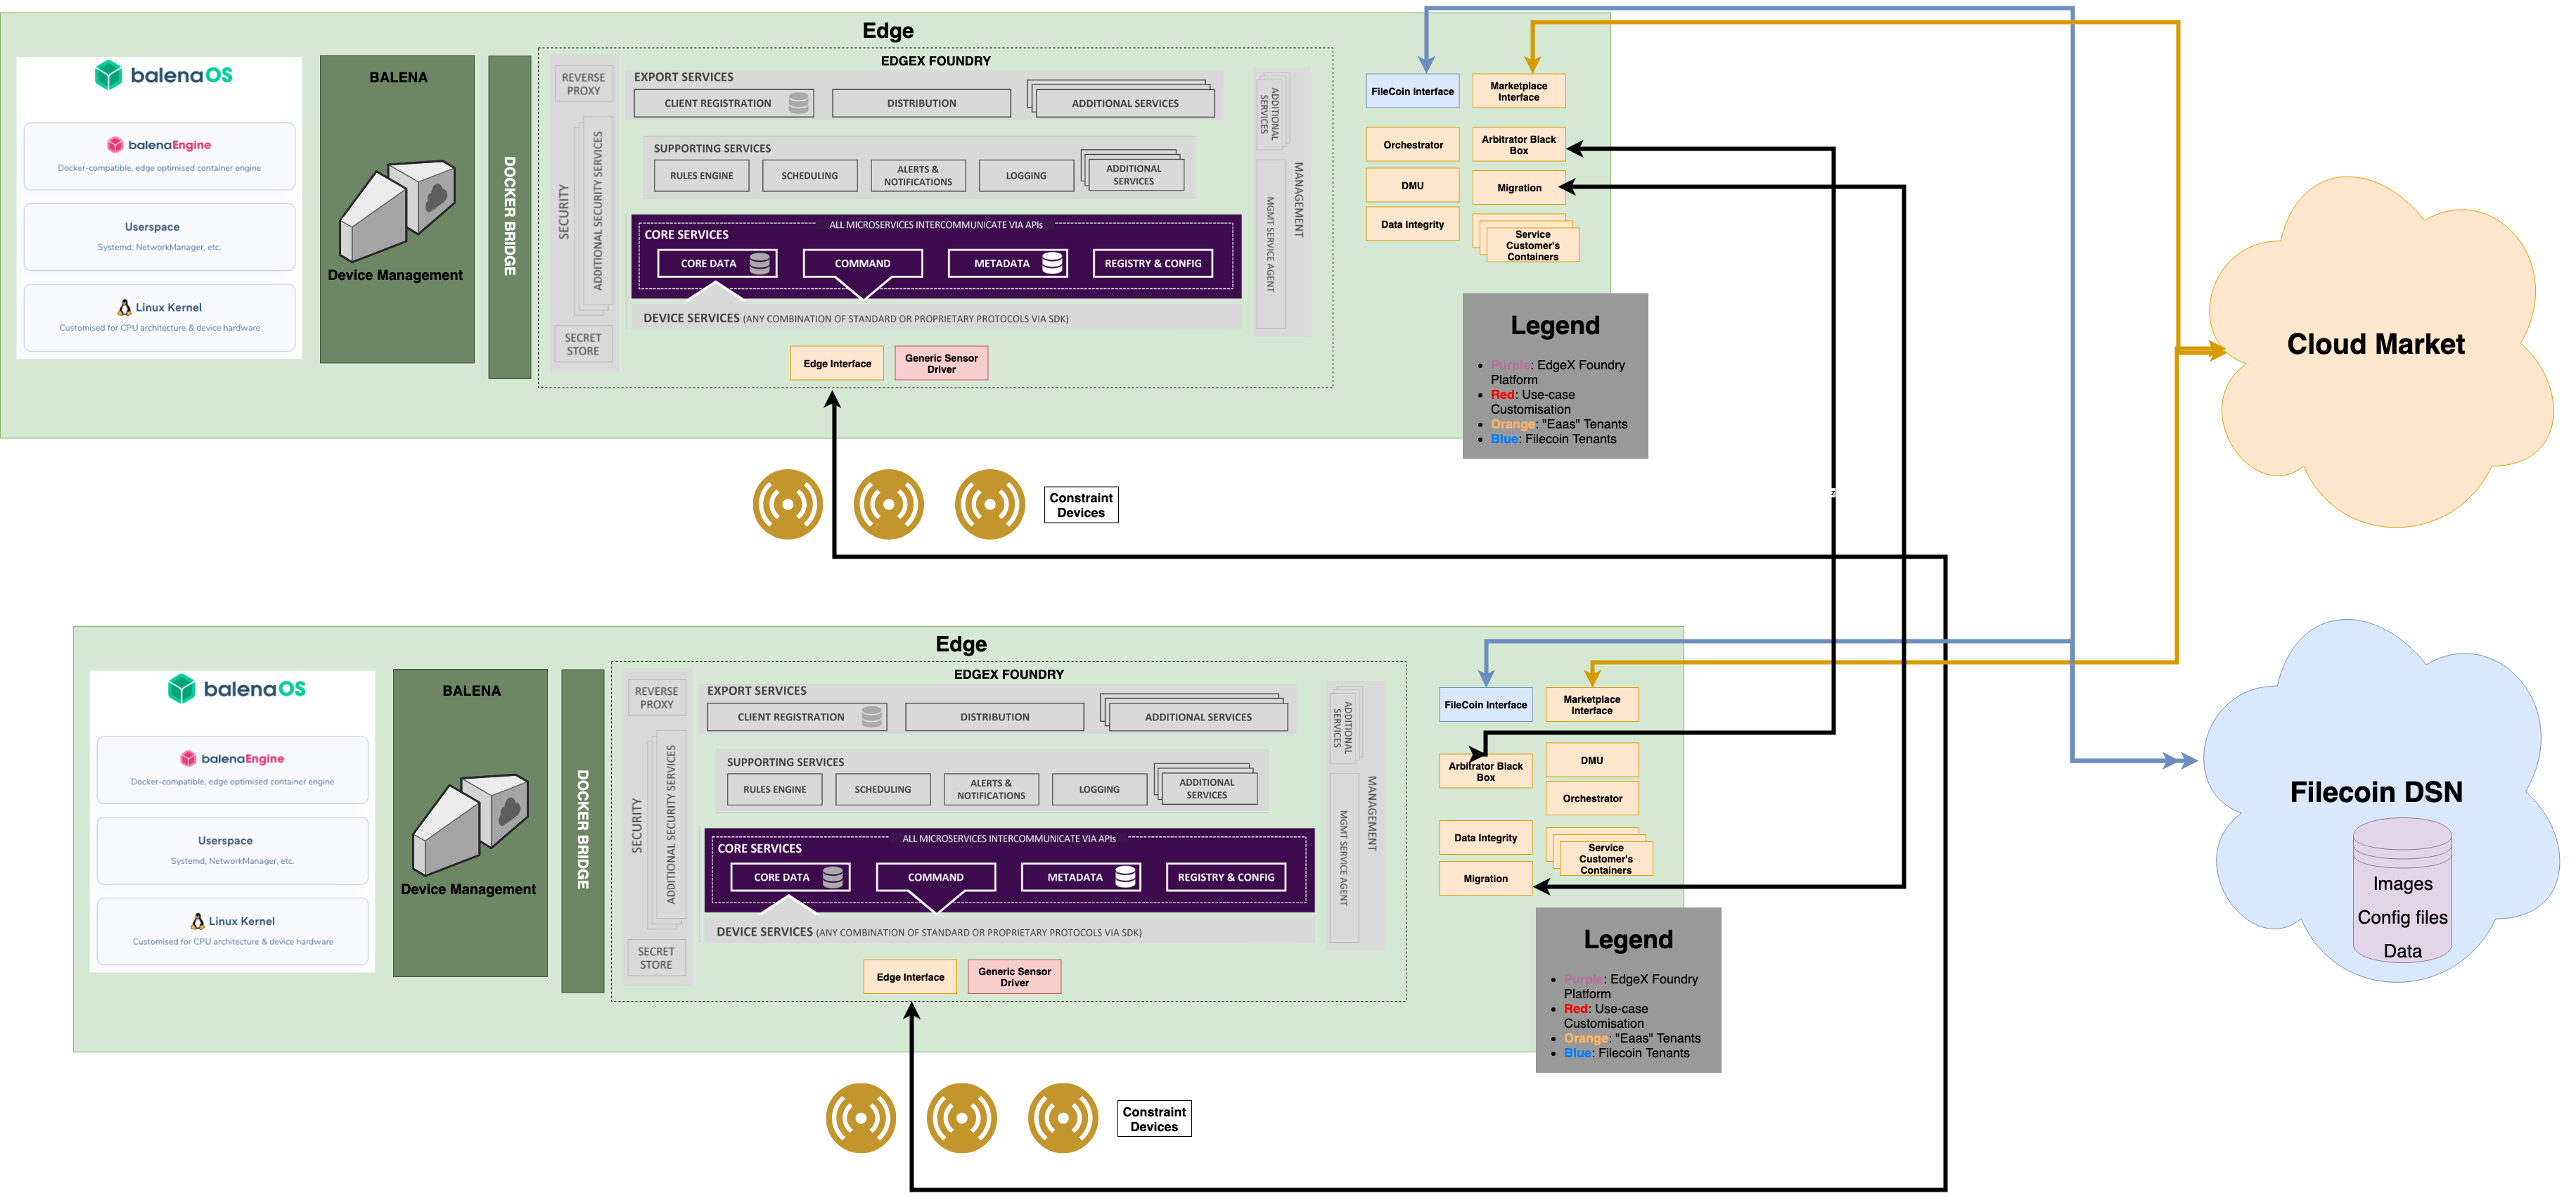
\includegraphics[width=0.9\textwidth]{images/EdgeEdgeArch_v2.png}
    \caption{Diagram showcasing the communication between microservices of different IoT Edge devices}
    \label{fig:edge2edge}
\end{sidewaysfigure}
\clearpage
\section{Communication Principles}
\subsection{IoT Edge to Edge}

In the proposed design, the IoT Edge devices are able to communicate automatically, in order to collaborate, offer insurance policies and even exchange resources for value.
 
The intercommunication is conducted through the south bridge of the Edge, using the Edgex platform as interface. As Edgex is hardware and protocol agnostic, the architecture enforces this paradigm and the interface will not be tied to a specific hardware protocol solution. It is expected to use a wireless protocol (e.g NB IoT, cellular data, WiFi, etc.) with certain (\textit{R})ange, \textit{(B)}andwidth, \textit{(P)}ower \textit{(C)}onsumption \textit{(R, B, PC)} requirements, featuring a different set of \textit{(R, B, PC)} according to the specification for each use-case and IoT Edge capabilities. The Interface module is built according to the Device Service specification of the Edgex platform using their SDK.
 
In essence, the interface module is the low-level connectivity layer of the Edge to Edge communication. It will expose a REST interface to the rest of the services that are interested in communicating with other IoT Edge devices, effectively acting as a gateway and reverse-proxy.

By abstracting the communication protocol, the architecture enables interoperability between the same IoT Edge modules and completely different communication protocols, depending on the use-case and the IoT Edge devices.

Figure \ref{fig:edge2edge} gives an impression on the communication between Edges. The arrows connect the submodules or subsystems that are expected to communicate using HTTP requests and RESTful APIs. For example, the Filecoin interface module is expected to communicate directly with the Filecoin network. Arrows that pass through the IoT Edge Interface indicate that they use the interface as a gateway.
\subsection{Cloud to Edge}

Each microservice in the IoT Edge platform has a corresponding one situated at the Cloud, which performs the same functionality. These two are expected to communicate directly. For example, EdgeX and DeviceHive have the same functionality in their respective systems, as platform managers performing the reference IoT activities related to the aggregated IoT data, thus they communicate directly.

Figure \ref{fig:cloud2edge} shows the communication between an IoT Edge and it’s corresponding Cloud, the arrows connect the submodules or subsystems that are expected to communicate using HTTP requests and RESTful APIs.
\clearpage
\begin{sidewaysfigure}
    \centering
    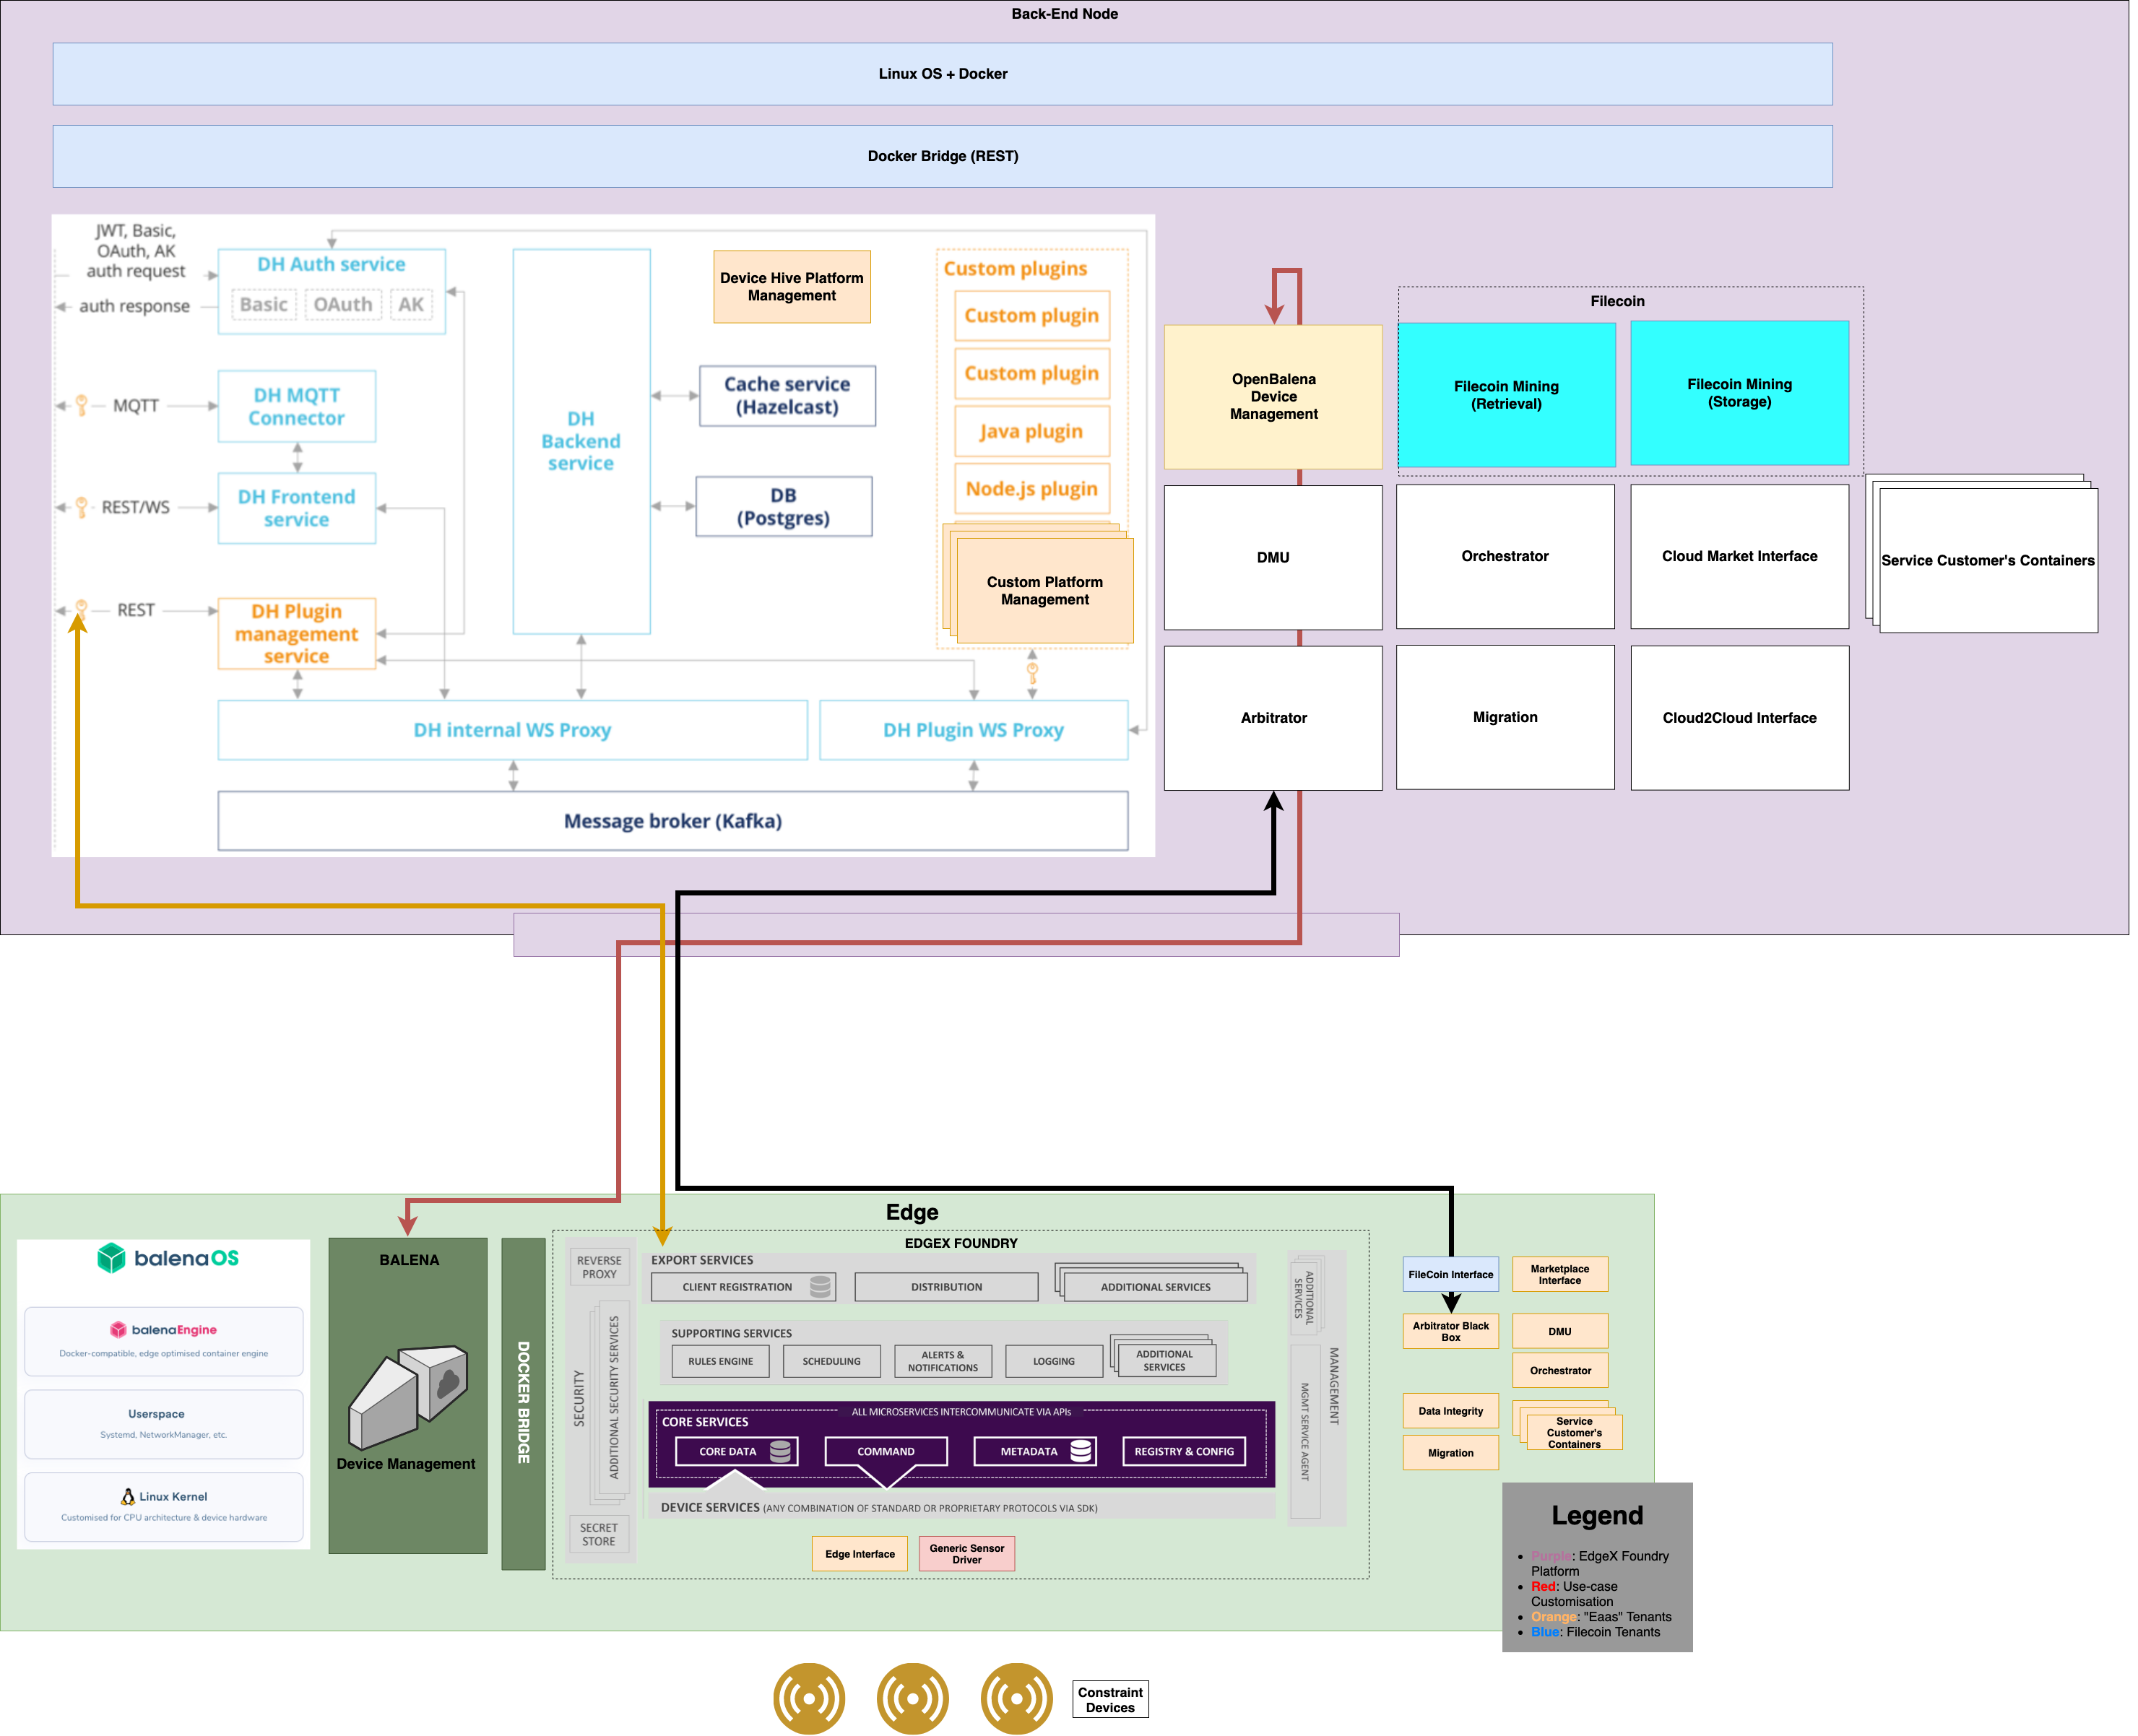
\includegraphics[width=0.7\textwidth]{images/CloudEdgeArch_v4.png}
    \caption{Diagram showcasing the communication between microservices of an IoT Edge device and it's parent Cloud}
    \label{fig:cloud2edge}
\end{sidewaysfigure}

\begin{sidewaysfigure}
    \centering
    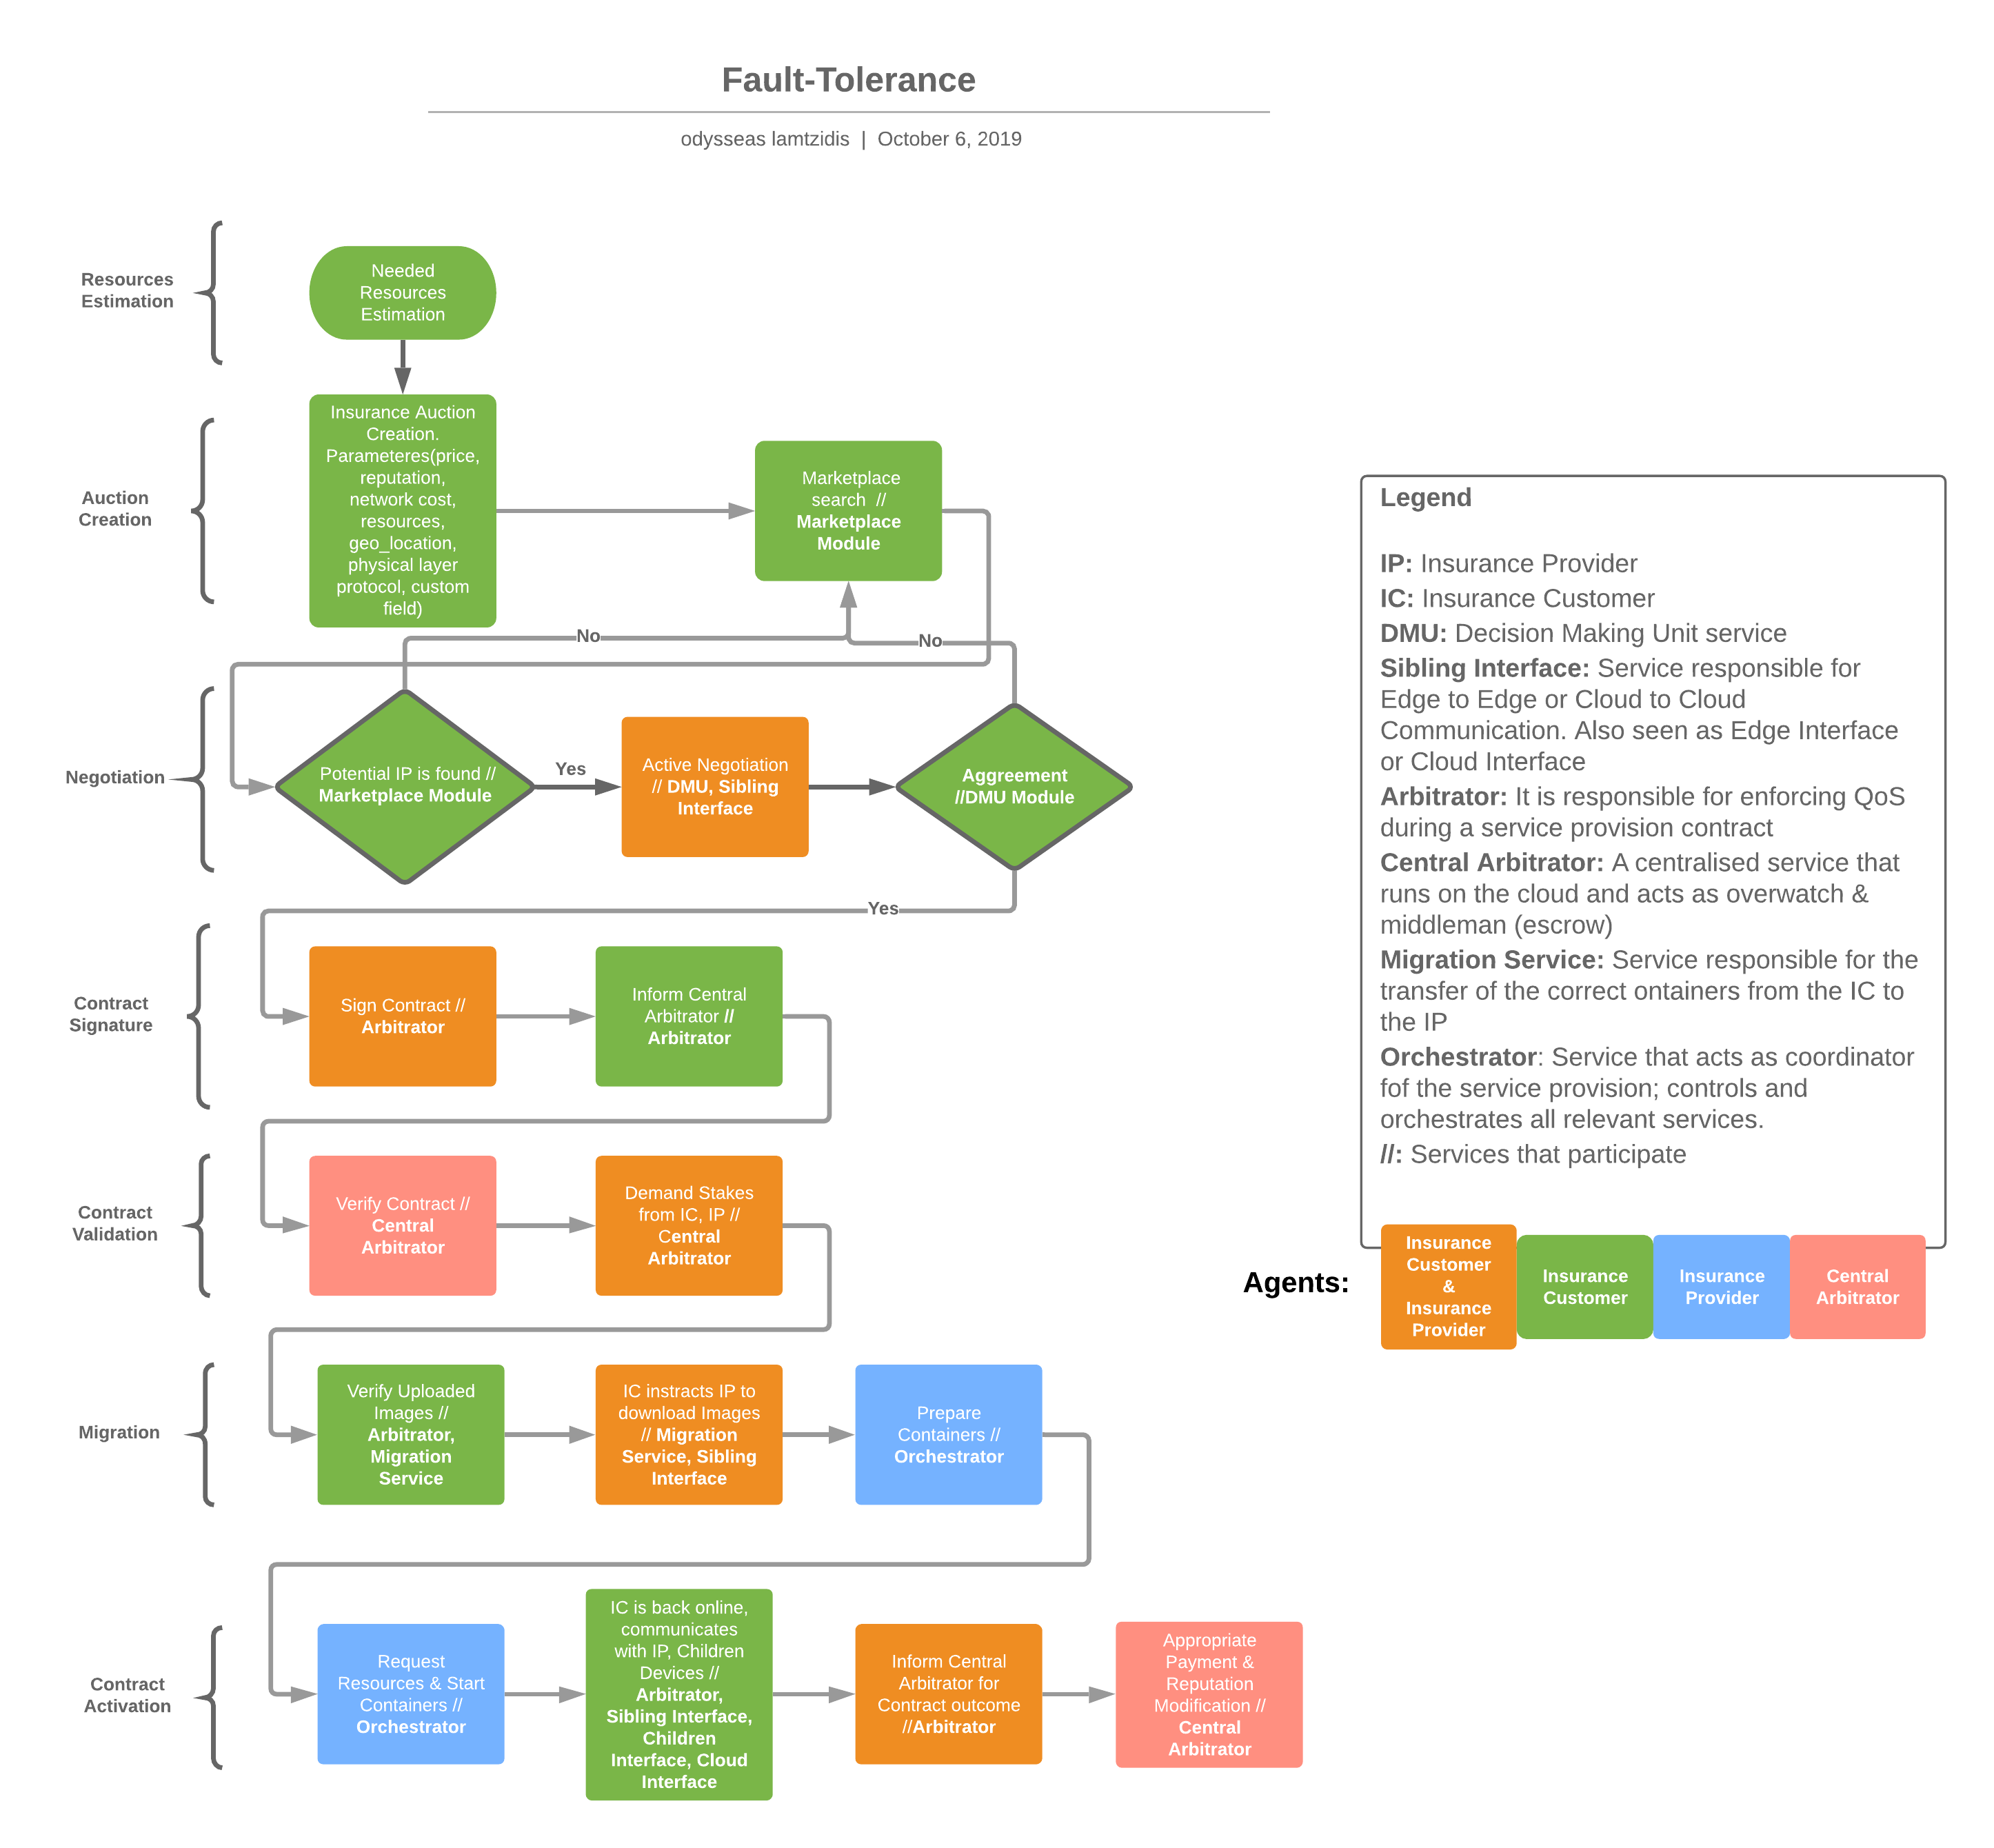
\includegraphics[width=0.8\textwidth]{images/fault_tolerance.png}
    \caption{The Fault-Tolerance reference process}
    \label{fig:fault-tolerance-process}
\end{sidewaysfigure}
\clearpage
\section{Fault-Tolerance High-Level Process at the IoT Edge Layer} \label{st:fault-tolerance}

\subsection{Overview}
In this section we aim to give a gist of the process we envisage for the fault-tolerance scenario, but which can be applied for the more generic \acrfull{eaas} as well. The activity description is not intended as an algorithmic definition, but rather as a high-level presentation of our approach. 

The IoT Edge Node accesses a central marketplace in order to find service-providers. Because of the nature of the fog paradigm, each IoT Edge is interested in systems that are near geographically (from a couple of meters to some kilometres, per the problem domain). Depending on the functionality of the Edge, it is possible that it requires the service-provider to have direct access to it’s sensors (via LoRa, BLE, Zigbee, etc.), which in turn dictates the proximity between the two IoT Edge Nodes. After finding a suitable Edge, the service-provider \acrshort{dmu} service is responsible for handling the negotiation and reaching an agreement.

Let IoT Edge device EdgeA which functions as an insurance customer and has reached an agreement with EdgeB for an insurance contract with certain attributes.
 
Based on the agreement, the service-providers Arbitrator Black Boxes of  EdgeA and EdgeB sign a contract and notify the Central Arbitrator \& the Cloud service-customer Arbitrator. The Arbitrators are responsible for performing \acrfull{qa} on exchange of value/services and perform payment for either honoring or breaching a contract. Since the service, that is being provided in this use-case is an insurance, we will define the service-provider and service-customer as an \textit{insurance-provider} and an \textit{insurance-customer}.

The workflow of an IoT Edge device that requests fault-tolerance services is depicted in Figure \ref{fig:fault-tolerance-process}.
 
By using a hybrid P2P/centralised model, the Arbitrators will be able to reach a consensus in case of breach of contract and perform the needed payment. We assume that the services outlined in the diagram and are shipped as part of the software solution are tamper-proof and thus trusted. They could however exist in a hostile  IoT Edge environment, where additional services actively attack the core package to enforce malicious behavior.  Security audit is out of the scope of this thesis, as we intend to present the notion rather than formally describing it.
 
The handover of the IoT devices from EdgeA to EdgeB is conducted via sending the appropriate containerized services (i.e device services, pre-processing services, etc. ) from EdgeA to EdgeB and then kick-starting those services when the contract is activated.

\textbf{Central Arbitrator:} A centrally run service which verifies the contracts and offers escrow services for payment between stakeholders. It communicates directly with the arbitrator services of both IoT Edge devices \& Back End Nodes.

\textbf{Cloud service-customer Arbitrator:} The arbitrator services of the corresponding Back End service. It performs the same functionality as the IoT Edge Arbitrator.

\subsection{The Marketplace Model}

In the IoT Edge scenario, the problem domain is a location bounded one, since the insurance-provider IoT Edge devices must have connectivity to both the sensors and the insurance-customer IoT Edge device. In contrast with the cloud auction model, this model is consisted of many local markets that function independently but are listed in a single marketplace for enhanced ease of access.
 
At this point, one could argue that probing locally for insurance-providers and using known standard IoT connectivity  protocols, is easier than reaching a central marketplace, finding an appropriate entry and then performing the connection through conventional internet access IPv4/IPv6 (i.e cellular connection, WiFi, Ethernet, etc. ). We believe that this process will be hindered by the inability of most protocols to perform adequately in regards to throughput. While these protocols are optimal for the communication between the sensors and the IoT Edge devices, they are not probably optimal for the Edge to Edge connection.
 
The auction model can be N:1, 1:N or N:M, we choose the latter because it is the most flexible. At any time t1, N IoT Edge devices are able to function as insurance providers and auction their services to potential insurance customers. At the same time, M insurance customers IoT Edges are able to auction a contract for providers to fill.
 
The \acrfull{qos} between the IoT Edges is ensured by the black-box arbitrators which function in good faith since they are considered tamper-proof by the system stakeholder. A centralized service is offered by the \gls{system-provider} to ensure QoS for all the cloud and edge stakeholders. It offers a full-range REST API for IoT Edge to post/update auctions, export statistics or issue custom contracts.
 
The procedure is as follows, (microservices that appear in the architecture as modules are in \textit{italics}). The procedure is organized and orchestrated by the \textit{orchestrator} module that is responsible for the smooth operation.

It consists of phases:
\begin{enumerate}
    \item Resources \& Cost Estimation (Required, Offered)
    \item Auction Creation
    \item Negotiation
    \item Contract Signature
    \item Contract Validation
    \item Migration
    \item Contract Activation
\end{enumerate}

\subsection{Resources and Cost Estimation Phase}

\noindent
\textbf{Insurance Customer:}
The service \textit{Decision Making Unit} (DMU), based on specific and industry state of the art algorithms, in case of customer, performs an estimation of the needed resources. Resources are categorized by industry standard terminology (RAM, CPU, cores, Storage, Bandwidth, Uptime, Network interfaces).

\noindent
\textbf{Insurance Provider:}
At this phase, the \textit{Decision Making Unit} (DMU) of the insurance provider determines the resources (RAM, CPU, Storage, Bandwidth, Uptime, Network interfaces) which will be auctioned in the insurance marketplace.
 
Both Insurance Providers \& Customers formulate an estimation of the preferred value for which they wish to sign the contract based on multiple factors, such as user preference. The final value will be determined in the negotiation phase.

\subsection{Auction Creation phase}
Using the IoT Edge Market REST API, IoT \textit{Edge market interface} issues an auction, detailing the resources needed/offered and other contract details, such as : price, reputation, network cost, geographic location, connectivity layer protocol and other custom fields. During setup phase, the IoT Edge scans for nearby Edges and requests for service-providers by issuing an insurance auction, using common IoT Protocols according to a configuration file (LoRa, BLE, Zigbee, etc.) via \textit{the Edge-to Edge interface}. Moreover, it can scan for IoT Edge devices which are geographically near and communicate using a standard Internet connection, to do this, it uses a centralized IoT Edge Marketplace.

\subsection{Negotiation phase}
After a match is found, the service informs the IoT Edge devices which then continue the negotiation of the offer/demand by using the \textit{DMU} and \textit{IoT Edge Interface}. Web-sockets and a REST API are model protocols for real-time communication. During the negotiation, the IoT Edge devices communicate in order to reach an agreement on the resources and the value that will be staked in the contract. Each IoT Edge can follow it’s own strategy but a reference can be given following a simple rule-based system.

\subsection{Contract Signature phase}
When an agreement has been reached (concerning the contract’s parameters), the IoT Edge \textit{Arbitrators} Black Boxes digitally sign a contract by staking a predetermined amount of value\footnote{Value is arbitrary, can be monetary value, cryptocurrency value, value in services.} and then inform the central Arbitrator of the event. We envisage a mechanism that will be able to perform an irreversible action in order to model the stake of value. A simple idea would be to use already established cryptocurrency projects that support such a functionality (e.g multi-signature addresses).

These microservices are expected to work as tamper-proof black boxes and thus are modeled to be trusted and non-hostile. The \textit{arbitrator} black boxes between IoT Edge devices communicate through the IoT \textit{Edge Interface} and directly with the central Arbitrator. We expect a proper threat model to be presented and a security analysis to be conducted, but we project that the arbitrator will \textit{usually}\footnote{The security analysis and the algorithmical structure of the arbitrator will give as the specification on top of which we will structure the technological stack} function as intended.


\subsection{Contract Validation phase}
The central arbitrator verifies the validity of the signed contract and then proceeds to add it in the active contracts list. The Central Arbitrator demands the stakes from the stakeholders in order to finalize the verification and acts as an escrow for the exchange of value/services.

\subsection{Migration phase}
As presented in Section \ref{st:balena-filecoin}, the IoT Edge stores locally the entirety of application logic, in the form of container images loaded into balenaEngine.

After the contract signature, the Insurance Customer \textit{arbitrator} informs the \textit{migration service} to verify the validity of the system images that are uploaded in the fillecoin DSN and update them as needed. After the verification, the insurance customer’s \textit{migration service} procures the needed keys to the insurance provider’s \textit{migration service} in order to find and download the images from the Filecoin DSN network. The communication with the Filecoin DSN is conducted through the \textit{filecoin interface} service. After download, the \textit{orchestrator} makes all the necessary container setups. 

\subsection{Contract Activation phase}
In case of critical failure, the insurance provider IoT Edge must be informed immediately in order to kick-start the containers and provide the insurance policy in a timely manner. The alert will be given by the insurance customer \textit{arbitrator} if possible or will be detected by the insurance provider.
 
The service provider's \textit{orchestrator} will request resources and spin up the Insurance Customer’s containers. The Service Provider’s \textit{arbitrator} is responsible for ensuring QoS in the insurance-provider  ’s operation according to the signed contract.
 
When the Insurance-customer comes back online, it’s \textit{arbitrator} communicates with the \textit{arbitrator} of the insurance provider, constrained devices and the insurance customer Cloud \textit{Arbitrator} in order to cross reference that operation went smoothly (i.e data analytics performed, data logged \& keys updated, no packet was lost)
 
The service provider's Arbitrator then proceeds to inform the central arbitrator of the certail contract activation, whether the contract was honored or not and finally the central arbitrator performs the appropriate payment and returns the stake to the party that got paid. In this scenario, each stake is the agreed payment, thus if the contract is voided, the insurance provider’s stake is given to the customer and his reputation is reduced or the provider receives the stake of the customer (as payment) and his reputation is increased.


